\documentclass[16pt]{book}
\usepackage{algorithm}
\usepackage{algpascal}
\usepackage{algpseudocode}
\usepackage{alltt}
\usepackage{amsmath}
\usepackage{amssymb}
\usepackage{caption}
\usepackage{float}
\usepackage{fontspec}
\usepackage{geometry}
\usepackage{graphicx}
\usepackage{hyperref}
\usepackage{parskip}
\usepackage{subcaption}
\usepackage{tabularx}
\usepackage[backend=biber, citestyle=numeric, sorting=none]{biblatex}
\addbibresource{sxfst.bib}
\addbibresource{vde.bib}
\addbibresource{thesis.bib}

\DeclareCaptionType{equ}[][]

\setmainfont{Noto Sans}
\hypersetup{urlcolor=blue, linkcolor=black, citecolor=black, colorlinks=true}


\begin{document}
\title{\textbf{Two Strategies for Engineering Herbicide Detoxification Enzymes}}
\author{James Engleback}
\maketitle
\tableofcontents

\chapter{Introduction}
\section{Abstract}

This thesis develops two enzyme engineering methods.
Both centre around developing a mutant of the bacterial Cytochrome P450 BM3 to hydroxylate the herbicide mesotrione at carbon $C_5$ for use in herbicide-resistant crop engineering projects.

Work was done in the Manchester Institute of Biotechnology under supervision of Prof. Andrew Munro and later Dr. Sam Hay.
The project was funded by the BBSRC iCASE program in partnership with agricultural technology company Syngenta.

\textit{Virtual Directed Evolution (VDE)} is a program developed to engineer enzymes with target performance in simulation using black box optimization algorithms.
Simulations model an enzyme sequence \textit{fitness} in a user-defined \textit{task} and returns a score.
A black box function optimizer is used to find progressively higher-scoring protein sequences.

In this case, the \textit{task} involves:

\begin{enumerate}
	\item Protein structure prediction from input sequence (side-chain repacking)
	\item Prediction of likely protein-mesotrione binding conformations (molecular docking)
	\item Score based on favourability of mesotrione binding and the sequence distance from BM3 template.
\end{enumerate}

The sequence:score information is passed to the optimizer and a new batch of protein sequences is generated and evaluated.
Genetic algorithms and Bayesian optimization are compared as optimization functions.

Once running, the process is fully automated.
Simulations are run in parallel and at scale on cloud infrastructure.
Here, throughput is 10\textsuperscript{4} mutants per day on a 50 CPU virtual machine.
Several methods of generating protein libraries for lab testing are presented.

\textit{Screening Fist} is an enzyme-substrate screening operation directed by an learning algorithm.
The screen detects binding activity between a purified enzyme and a compound screening library.

Screening data is passed to an agent to fine tune its internal, pre-trained model of protein function from sequence, which is used to virtually screen BM3 mutant sequences for predicted binding to mesotrione.
The model can also be used to estimate the information gain ($\mathbb{E}IG$) of a candidate batch of experiments based on its uncertainty, which can be used for optimal design of subsequent screens.
The end use of the model is to generate useful predictions of protein function from sequence in downstream enzyme engineering tasks.

A high throughput binding assay is developed, including software to automate test design, liquid handling and data analysis.
Five purified BM3 mutants are screened against a chemical library of ~ 900 FDA-approved drugs, some of which share common features with herbicides.

An agent containing a multi-task deep neural network is constructed and trained to functionally annotate an input protein sequence and estimate its likelihood of interacting with a particular compound.

Pre-trained from a custom database of ~ 10\textsuperscript{6} annotated protein sequences and their known ligands, the model is retrained on screening data, evaluated for accuracy and used to generate new BM3 mutants with predicted mesotrione binding capabilities.

\section{Introduction}
By 2050, global food demand will increase by a projected 70\% compared to 2009 \cite{food2009high}. 
12\% of the Earth’s ice-free land is already cultivated for crops and the potential for expanding this area is limited \cite{licker2010mind}\cite{food2009high}.
 
The ‘yield gap’ is the difference between the predicted maximum yield of a given crop in a given area, and the actual yield in that area. 
Yield gaps are often largest in under-developed agricultural systems that lack suitable irrigation, chemical fertilizer and crop protection \cite{licker2010mind}. 
The most significant contributor to yield loss is weeds, which can reduce yields by up to 80\% in some crops if no action is taken \cite{oerke2006crop}. 

Herbicides kill weeds by disrupting key metabolic processes in the plant. 
No new classes of herbicide have been developed since 1998, whilst multiple-herbicide resistant ‘superweeds’ are a growing problem worldwide \cite{norsworthy2012reducing}. 
High application rates of multiple mechanisms of action is an effective strategy to manage herbicide resistant weeds, but is limited by the crops’ intrinsic tolerance to the herbicide treatments.


Crops with engineered multiple herbicide resistance are the most effective weed management strategy since they allow high application rates of multiple classes of herbicide, minimising the probability of herbicide resistant weed outbreaks \cite{green2012benefits}. Herbicide resistant crops are generated by:
\begin{enumerate}
	\item Target site resistance: In this case the crop is transformed with an enzyme with the same biochemical function as the herbicide target site, but is not herbicide-sensitive, creating a ‘metabolic bypass.’
	\item Metabolic enhancement: Crops can be transformed with enzymes that degrade herbicides into a non-phytotoxic product.
\end{enumerate}

\subsection{HPPD Herbicides}
4-Hydroxyphenylpyruvate Dioxygenase (HPPD, EC1.13.11.27) is an important herbicide target and an area of interest for generating herbicide resistant crops. 
HPPD inhibitors are commonly deployed in cereal crops, which tolerate HPPD inhibitors better than broadleaf weeds and therefore allows preferential toxicity towards weeds. 
HPPD inhibitors are the last class of herbicides to have been discovered and are popular because of the broad spectrum of weeds that they are toxic to and because they can synergise with other herbicides, leading to the development of herbicide mixtures that allow greater application flexibility and minimise the chance of weeds developing herbicide resistance \cite{kaundun2017mechanism}.


HPPD is ubiquitous to aerobic organisms and catalyses the transformation of 4-Hydroxyphenylpyruvate to homogentisate, an important step in tyrosine catabolism \cite{moran20054}. In plants, homogentisate is a precursor to both plastoquinone and α tocopherol \cite{soll1980tocopherol}. 


Plastoquinone is an essential cofactor for the synthesis of carotenoids and in the coupling of photosystem I and II. 
Carotenoids are accessory light harvesting pigments that prevent generation of ROS by quenching high energy triplet-state chlorophyll b. 
Additionally, β-carotene is a structural element of the photosystem II core, depletion of β-carotene causes the release of chlorophyll which is phototoxic in its free state \cite{kramer2007modern}. 
Damage from HPPD-inhibition is exacerbated by depletion of α tocopherol, an important amphipathic antioxidant that quenches reactive oxygen species generated during uncoupled photosynthesis and scavenges lipid peroxyl radicals \cite{munne2005role}.
 
\subsubsection{HPPD Inhibitors}
All known potent HPPD inhibitors contain a 1, 3 diketone moiety \cite{kaundun2017mechanism}. 
The crystal structure of tobacco (nt) HPPD with an experimental diketone inhibitor \textit{(DAS869)} bound revealed that octahedral coordination of the catalytic Fe\textsuperscript{2+} was required for tight binding \cite{yang2004structural}. 
Binding is also mediated by π-stacking of the benzoyl moiety of the inhibitor between two phenylalanine residues in the binding pocket.


HPPD inhibitors can be identified in vitro high throughput screens, such as that described by \cite{yang2004structural} who used a partially purified homogentisate dioxygenase from Achromobacter xylosoxidans to couple homogentisate production to maleylacetoacetate. 
Production of maleylacetoacetate results in an increased absorbance at 300 nm, allowing the assay to be carried out in a microtiter plate and tracked by a plate reader. 
A more recent advance in HPPD-inhibitor screen is a bacterial bioassay \cite{rocaboy2014novel} that takes advantage of the accumulation of a brown melanin-like pigment in E. coli cells that overexpress a plant HPPD gene; incubation with a potent HPPD inhibitor prevents the formation of the melanin-like pigment and allows determination of IC50 accurate in the sub-micromolar range.


Maize can rapidly metabolize HPPD inhibitors like mesotrione, which allows farmers to use this class of inhibitor as a selective herbicides \cite{hawkes2001mesotrione}. 
The essential role of cytochrome P450s in herbicide metabolism was elucidated by co-application of mesotrione with the P450 inhibitor malathion, and the subsequent discovery of the 4-hydroxy-mesotrione metabolite \cite{hawkes2001mesotrione}. 
Outbreaks of mesotrione-resistant weeds \textit{(Aramanthus spp.)} 
have appeared in continuous corn seed production fields which have received repeated low doses of the herbicide \cite{hausman2011resistance}. 
Like corn, the mesotrione-resistant Aramanthus spp. tolerated high doses of the herbicide via metabolic inactivation by 5-hydroxylation of mesotrione, which suggests that a P450 may be responsible \cite{kaundun2017mechanism}.


\subsubsection{HPPD-inhibitor Resistant Crops}
In 2013 a Syngenta and Bayer submitted a transgenic soybean \textit{(Glycine max L.)} dubbed the \textit{MGI Soybean} with engineered HPPD-inhibitor tolerance for regulatory review \cite{syngenra2013mgi}. 
This represents an important technology for farmers, since in the major maize-growing areas of the United States (the ‘Corn Belt’) maize crops are immediately followed by Soybean in 75\% of cases \cite{hawkes2007ep}.
Soybean is extremely sensitive to residual HPPD-inhibitors that may persist in the soil, so it is important to produce a variety of Soybean that can tolerate this class of herbicide to allow safe crop rotation and herbicide application flexibility.


In 2007, Tim Hawkes’ team at Syngenta filed patents in the US, Europe and China for several genes that were capable of conferring HPPD-inhibitor resistance to otherwise susceptible crops \cite{hawkes2007ep}.
One of the patented genes was an HPPD variant cloned from wild oats \textit{(Avena fatua)} which is mildly tolerant towards HPPD-inhibiting herbicides. 
The gene was subject to a combination of site-directed mutagenesis, random mutagenesis and gene shuffling. 
The resultant mutants were screened by transformation into E. 
coli cells plated on media supplemented with tyrosine and an HPPD-inhibiting herbicide in similar stead to the aforementioned bacterial bioassay for HPPD inhibitors  \cite{rocaboy2014novel}. 
Colonies that accumulated a melanin-like pigment in the presence of the herbicide were considered to be herbicide-tolerant.


To further the level of herbicide tolerance in the proposed line of Soybean, Hawkes’ team identified several putative P450s capable of metabolising herbicides by comparing quantitative trait loci (QTLs) from inbred lines of maize that had differing levels of tolerance to HPPD-inhibitor mesotrione and acetolactate-synthase inhibitor nicosulfuron.  
Expression and analysis of bacterial artificial chromosomes generated from the QTLs yielded a P450 with activity towards nicosulfuron (‘Maize NSFL’) and one with activity towards mesotrione (CYP72A1). 



The CYP72A family of P450 monooxygenases have a broad range of biological functions in plants, though a phylogenetic analysis by \cite{prall2016utility} revealed insights into the functional regions of the enzyme family such as the substrate recognition regions, they also found that enzymes in this family can be modelled onto the human CYP3A4 structure with a relatively high predicted accuracy, which may be a useful tool for producing mutants of this enzyme.
 
 
 The patent also covers CYP81A6 from rice \textit{(Oryza sativa L.)}, 
 which had been previously discovered to confer tolerance to benzaton - a photosystem II inhibitor, and to the sulfonylurea class of acetolactate synthase inhibitors \cite{zhang2007identification}. 
 The product has not yet reached the market.



Monooxygenation of herbicides by P450s is an important mechanism by which crops tolerate herbicides \cite{siminszky2006plant}. 
P450-mediated degradation of herbicides can be enhanced in crops by the application of chemical ‘safeners’ to the seed coat or as a foliar spray. 
Safeners like naphthalic anhydride induce expression of certain gene clusters that tend to include P450s capable of herbicide metabolism \cite{davies1998mode}. 


Insertion of an oxygen into a herbicide can be sufficient to detoxify it in itself, as in the case of mesotrione \cite{kaundun2017mechanism}.
In other cases, hydroxylation of the herbicide is followed by conjugation with a bulky, hydrophilic molecule, such as glutathione and its subsequent export from the cytosol into the vacuole or periplasm via an ABC transporter \cite{yuan2007non}. 
In addition to the aforementioned MGI soybeans, exogenous P450s have been used to confer herbicide tolerance to rice \textit{O. sativa} \cite{kawahigashi2005enhanced}\cite{kawahigashi2008transgenic}, potatoes (\textit{Solanum tuberosum})\cite{inui2005herbicide}, tobacco \textit{(N. tabacum)} and A. thaliana \cite{didierjean2002engineering}.

\section{Overview of This Work}

This thesis aims to engineer a cytochrome P450 capable of $C_5$ hydroxylation of the HPPD inhibiting herbicide mesotrione.
Within that, it also aims to develop new computer-assisted protein design methods with applications beyond the previous aim.
One method is based around a machine learning model designed to predict the likelihood of a binding interaction between an input protein sequence and chemical structure,
The other is virtually analogous to directed evolution, evaluating the \textit{fitness} of mutants by simulation and managed by a genetic algorithm.

\chapter{Screening Fist}
\section{Abstract}
\textit{Screening Fist} is a screening operation used to train a machine learning model to predict the likelihood of a given enzyme binding to a given small molecule from sequence.
The model is pre-trained on a large and general dataset of protein and small molecule binding pairs scraped from several online sources before retraining on the screening data.
The screening data is generated in-house with a high-throughput, custom developed Cytochrome P450-small molecule binding assay, with which five P450 BM3 mutants were each screened for binding against 980 drug-like molecules.
\par
The retrained model can be used for virtual screening of new enzyme sequences against a specific target molecule, or to query a single sequence against many prospective small molecule binding partners.
It can also be used to design subsequent rounds of screening based on the expected information gain of an experimental design.

% ----------
\section{Introduction}

\subsection{Engineering Problem and Context}

Herbicide-resistant crops are important for global agriculture because they mitigate yield losses due to weeds and give farmers extra flexibility in their herbicide application programs, which is important to suppress emergence of herbicide-resistant weeds. % value statement
\par
Herbicides kill plants by inhibiting key metabolic processes and their species-specificity is determined by susceptibility of herbicide target and their ability to  metabolize the herbicide. % herbicide overview
HPPD inhibitors are a key herbicide class that cause leaf bleaching and death in susceptible plants. 
HPPD inhibition  disrupts tyrosine catabolism which disrupts UV-protection via carotenoid production and photosynthetic electron shuttling via plastoquinone, leading to death by UV damage and radical toxicity. % HPPDs
\par
Engineering HPPD-inhibitor resistance into plants have used the HPPD and metabolic enzymes from naturally resistant species like \textit{Avena fatua}. 
\textbf{note: ref this.}
CYP72A1 is a cytochrome P450 that initiates metabolism of HPPD herbicides by ring hydroxylation at $C_5$ and has been explored as a means of engineering HPPD herbicide metabolism into soybean.
\textbf{Figure \ref{mesotrione}} shows the chemical structure of mesotrione and its primary metabolite 5-hydroxy mesotrione. % cyp 72a1 & engineering attempts

\begin{figure}
	\begin{center}
	\caption{\label{mesotrione} The HPPD-inhibiting herbicide mesotrione and its primary metabolite 5-hydroxy mesotrione - hydroxylated at the $C_5$ position naturally in some plants by indigenous Cytochrome P450s, priming it for subsequent stages of detoxification.}
	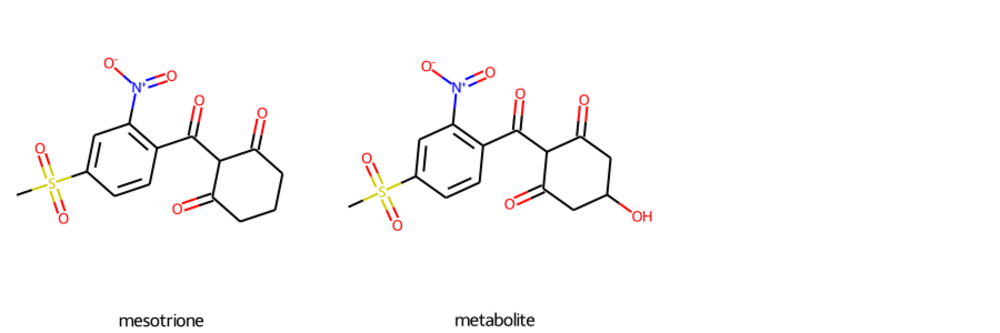
\includegraphics[width = \textwidth]{img/mesotrione+metabolite.png}
	\end{center}
\end{figure}

\par
\begin{figure}
         \begin{center}
         \caption{\label{mesotrione} The HPPD-inhibiting herbicide mesotrione and its primary metabolite 5-hydroxy mesotrione - hydroxylated at the $C_5$ position naturally in some plants by indigenous Cytochrome P450s, priming it for subsequent stages of detoxification.}
         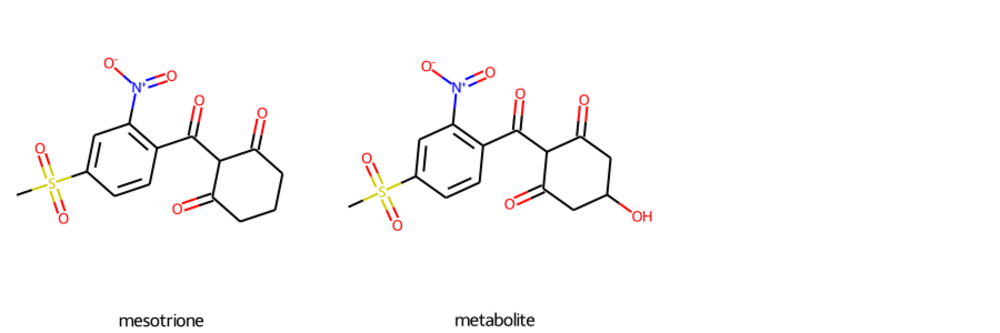
\includegraphics[width = \textwidth]{img/mesotrione+metabolite.png}
         \end{center}
 \end{figure}

 \par

Cytochrome P450s are a ubiquitous class of heme-dependent oxidoreductases that are frequently involved in xenobiotic metabolism. % p450s overview
Bacterial P450s have been engineered to catalyse a range of xenobiotic biotransformations. The bacterial P450 BM3 from \textit{Bacillus megaterium} is one such bacterial P450 whose structure has been studied extensively \cite{munro2002p450}. 


Notably, BM3 is a popular target for enzyme engineering studies, owing in part to its extensive documentation, ease of expression and \textit{evolvability} \cite{bloom2006protein}.
Some examples of BM3 mutants with altered substrate scope are shown in \textbf{Table \ref{bm3_table}} \cite{wong}.
\par

\begin{table}
	\begin{center}
		\caption{\label{bm3_table}Examples of engineered BM3 Mutants with altered substrate scope \cite{wong}}
		\begin{tabular}{l|p{3cm}|l}
		\textbf{Mutant} & \textbf{Substrate scope} & \textbf{Structure} \\
		\hline 
		F87A/I263A/(A328I) & Nootkatone & 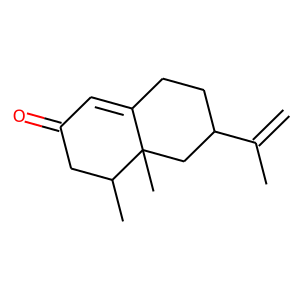
\includegraphics[width = 2cm, height= 2cm, keepaspectratio=true]{img/nookatone.png} \\
		A328F & Limonene & 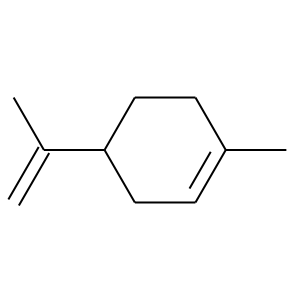
\includegraphics[width=2cm, height= 2cm, keepaspectratio=true]{img/limonene.png} \\
		R47L/Y51F & Alkylbenzenes (no heteroatoms) & 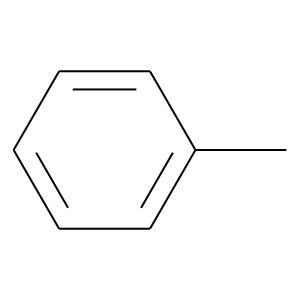
\includegraphics[width=2cm, height= 2cm, keepaspectratio=true]{img/alkyl-benzene.png} \\
			R47L/F87V/L188Q (LVQ) & Coumarins & 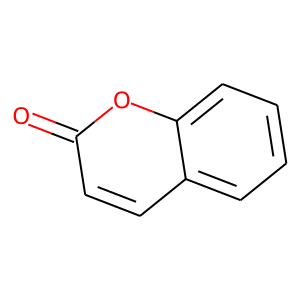
\includegraphics[width=2cm, height= 2cm, keepaspectratio=true]{img/coumarin.png} \\ % this pic sucks
			A74G/F87V/L188Q (GVQ) & Indole, Lovastatinn, beta-ionine, organophosphates, polyaromatic hydrocarbons, chlorinated dioxins & 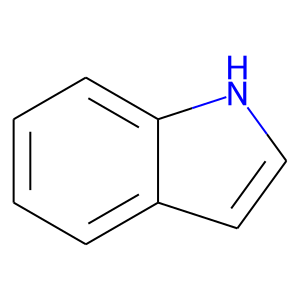
\includegraphics[width=2cm, height= 2cm, keepaspectratio=true]{img/indole.png} \\
	\end{tabular}
	\end{center}
\end{table}

The BM3 A82F/F87V mutant has a broad substrate specificity \cite{butler2013key}, and represents an attractive starting point for engineering altered substrate scope, however it has no binding activity towards the HPPD herbicide mesotrione. % bacterial p450 engineering
%%%%%%% find that spec

\subsection{Technologies Used}
\subsubsection{Machine Learning}
\subsubsection{Transfer Learning}

%Transfer learning is a phenomenon where a model trained on one task, can be re-trained on a different domain-related task  sample-efficiently compared to an untrained model.
%For example an object detection model trained from from images of vehicles can transfer efficiently to identification of cell phenotypes from microscopy images.
%This is because some learned features generalize well enough to be useful in other tasks, reducing the number is samples required to reach a baseline performance level.

Transfer learning is a popular approach to enhancing model accuracy and involves pretraining the model on a large, general dataset before transferring to a new task. 
The effect is a reduction in the number of samples required to train the model. 
Pre-training datasets do no necessarily need to be closely related to the target task, for example: models initially trained on the CIFAR 100 dataset (containing cars, animals etc) have been successfully re-tasked on phenotype identification from microscopy images \cite{ng2016nuts}. % xfer learning justification

In the domain of protein sequence-based machine learning, thoroughly pre-trained models are available for generating a neural embedding of a given protein that can improve sample efficiency in downstream learning tasks.
Generally, these models are large attention-based models trained \textit{unsupervised} on a large corpus of protein sequences, like the \textit{TrEMBL} collection of \textit{Uniprot}.
In this case, unsupervised training often entails reconstruction of a distorted or masked protein sequence and is run on hardware far beyond the budget of this project.

\subsubsection{The TAPE Benchmark}

\textbf{note: explain relevance, flesh out}

Tasks Assessing Protein Embeddings \cite{tape2019} is a benchmark for comparing numerical representations of protein sequence (learned or otherwise) on a set of biological learning tasks from different domains of protein science. 
It currently contains five tasks:

\begin{enumerate}
\item \textbf{Secondary Structure Prediction Task:}
\item \textbf{Structural Contact Prediction Task:}
\item \textbf{Remote Homology Detection:}
\item \textbf{Fluorescent Protein Landscape Prediction:}
\item \textbf{Protein Stability Landscape Prediction:}
\end{enumerate}

Tasks 4 and 5 are most applicable to protein engineering, since they involve metric prediction from a set of largely similar protein sequences.
The leader boards for performance on these two tasks as of 5 Jun 2022 are:

\textbf{Fluorescence:}

\begin{table}
	\begin{center}
		\caption{Fluorescence TAPE benchmark leader boards \label{tapefluor}}
		\begin{tabular}{l|p{3cm}|l}
			\textbf{Ranking} & \textbf{Model} & \textbf{Spearman's rho}\\
		\hline 
			 1. & Transformer & 0.68 \\
			 2. & LSTM & 0.67 \\
			 2. & Unirep & 0.67 \\
			 4. & Bepler & 0.33 \\
			 5. & ResNet & 0.21 \\
			 6. & One Hot & 0.14 \\
		\end{tabular}
	\end{center}
\end{table}


\textbf{Stability:}

\begin{table}
	\begin{center}
		\caption{\label{tapestab} Stability TAPE benchmark leader boards }
		\begin{tabular}{l|p{3cm}|l}
			\textbf{Ranking} & \textbf{Model} & \textbf{Spearman's rho}\\
		\hline 
			 1. & Transformer & 0.73 \\
			 1. & Unirep & 0.73 \\
			 1. & ResNet & 0.73 \\
			 4. & LSTM & 0.69 \\
			 5. & Bepler & 0.64 \\
			 6. & One Hot & 0.19 \\
		\end{tabular}
	\end{center}
\end{table}

\textbf{Facebook AI Research - Evolutionary-Scale Modelling}
\textbf{note: explain model architecture and purpose, set of pretrained models and availability}

\subsection{Related Work}

\textbf{note - do:}
\begin{itemize}
	\item \textbf{biswas}
\end{itemize}

\subsection{Overview of This Work}

This project is a proof of concept for a new approach towards enzyme engineering using machine learning.
Broadly speaking, it involves screening a number of enzyme mutants for activity towards a large number of compounds of interest.
This data is then used to train a machine learning model to predict the likelihood of activity between a given protein sequence and small molecule structure.
The trained model has two applications:
\begin{enumerate}
	\item Virtually screen a large number of potential protein and small molecule candidates for potential activity. 
		These screens can be used to explore potential substrate scope of a given protein, or as a virtual fitness function for use in virtual directed evolution - where a sequence optimization algorithm evaluates sequences against a fitness function.
	\item Optimal design of subsequent screening rounds based on the expected information gain ($EIG$) of a candidate experimental design.
\end{enumerate}

The specific approach in this project is to screen a local area of sequence space surrounding the wild-type P450 BM3 against a library of 980 FDA-approved drug compounds.
Drugs share chemical properties with herbicides so are suitable for a proof of concept study.

% ----------
\section{Methods and Development}
\subsection{Assay Development}

In order to generate a P450 BM3-specific dataset on which a model could be re-trained to make binding likelihood predictions on drug-like molecules, a high throughput P450 binding detection assay was developed.
The assay is based on traditional UV-Visible light spectroscopy-based techniques for detection of P450-ligand binding, miniaturized into a 384 well format. 
It relies heavily on automation and a throughput of 980 compounds per day is demonstrated.

\subsubsection{Aim}

The initial aims of this development work were:

\begin{itemize}
	\item Develop a high throughput P450-ligand binding assay based on established biophysical characterisation techniques.
	\item Develop necessary software for design and analysis of each assay.
	\item Compare the precision and accuracy of the assay to existing techniques.
\end{itemize}

\subsubsection{Basis: UV-Visible Spectroscopy for Monitoring Cytochrome P450-Ligand Binding}

The assay is based on a technique for quantifying P450-ligand interactions based on UV-visible photospectroscopy.
The technique consists of the purified Cytochrome P450 heme domain in question in a neutral buffer at around 5-10 µM in a optically clear cuvette.
Since only the heme-containing domain of the P450 is used, no chemical reactions are expected to take place which removes time-sensitivity from the assay.
\par

The UV-visible light absorbance of the sample is typically measured for all wavelengths between 200 and 800 nm, which for a P450 without a ligand bound in the active site should show a large and defined absorbance peak at around 420 nm.
\par
After an initial absorbance measurement of the ligind-free P450, the compound of interest can be titrated into the sample.
On binding to the ligand, the absorbance profile of the P450 changes such that the absorbance at 420 nm ($A_{420}$) decreases and absorbance at 390 nm ($A_{390}$) increases.
\par
The change in $A_{420}$ and $A_{390}$ in response to change in ligand concentration can be quantified and used to derive metrics that indicate affinity between the ligand and P450 using Michaelis-Menten kinetics models.
\par
The original Michaelis-Menten model of enzyme kinetics states:

\begin{equation}
	v = V_{max} \frac{[S]}{[S] + K_M} 
\end{equation}

where $v$ is the reaction velocity - the rate of an enzymatic reaction. 
$V_{max}$ is the maximum possible $v$ for this particular enzyme-substrate pair, $[S]$ is the concentration of the substrate and $K_M$ is the $[S]$ at which $v = V_{max}$.
\par
$V_{max}$ and $K_M$ are useful metrics for quantifying the binding interaction between enzyme and substrate, where low $K_M$ indicates a tight binding interaction and a high $V_{max}$ indicates a large magnitude of response.

Important assumptions in the Michaelis-Menten model of kinetics are:

\begin{enumerate}
	\item The concentration of enzyme is $< K_d$ 
	\item The rate of reaction is directly proportional to the concentration of the substituents
	\item The reaction is at chemical equilibrium at the time of measurement
	\item The interaction is reversible
\end{enumerate}

A variant of this model is applied to Cytochrome P450 photospectroscopy assays, where the response to a ligand is detectable in the 390-420 nm region.
Ligand binding to a P450 alters the electron environment in the heme, which changes the UV-Visible light absorbance profile.
Specifically, absorbance at 420 nm is reduced and absorbance at 390 nm increases.

In this case, $v$ is substituted for $\Delta A_{390} - \Delta A_{420}$ - the magnitude of the P450 response and $K_M$ is substituted for $K_d$ - the dissociation constant between the enzyme and ligand.
This yields the formula:

\begin{equation}
	Response = \Delta A_{390} - \Delta A_{420} = V_{max} \frac{[S]}{[S] + K_d} 
\end{equation}

An example of this is shown in \textbf{figure \ref{arachadionictitration}}, where the fatty acid arachadionic acid was titrated into a sample of P450 BM3 wild-type.

\begin{figure}
	\caption{\label{arachadionictitration} Response of P450 BM3 to Arachadionic Acid from a titration experiment, from which steady-state Michaelis-Menten kinetics can be derived. The legend shows the concentration of arachadionic acid in µM.}
	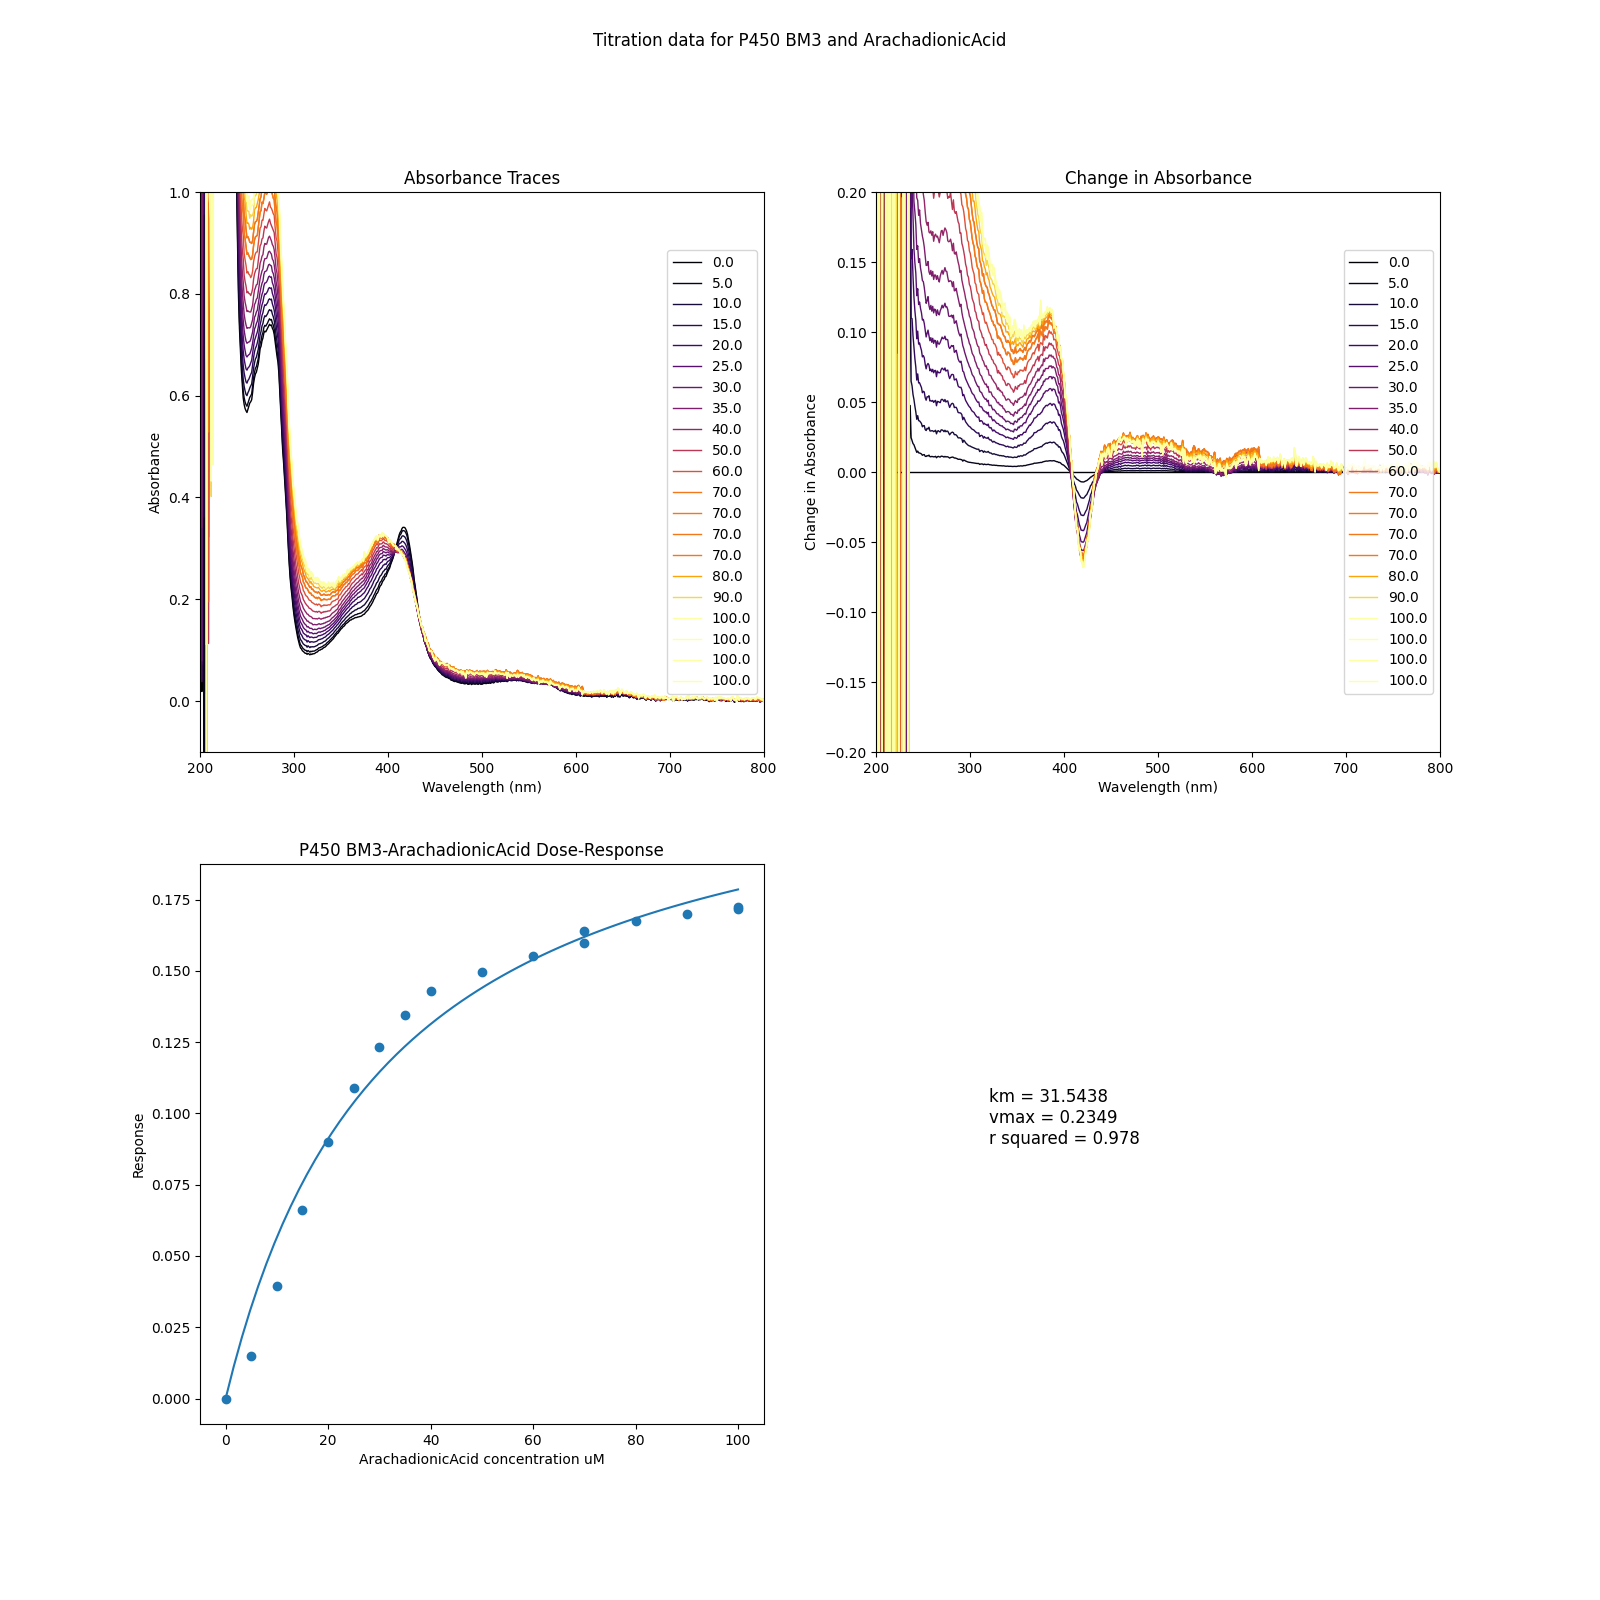
\includegraphics[width = \textwidth]{img/ArachadionicAcid.png}
\end{figure}

% -----------------

\subsubsection{Development}

This style of assay was miniaturized into a 384-well format for the purpose of this project.
The 384-well format permits high throughput screening of compounds for binding with a given P450 provided it is sufficiently stable to last the duration of the experiment without degrading and interfering with measurement.

% echo.py
At micro-scales, precision dispensing of both compound and protein is critical for overall assay precision.
To achieve sufficient precision, compounds were dispensed using an \textit{Echo 550} acoustic liquid handling device, which uses ultrasound to move liquid from a source plate to a destination plate.
In order to achieve the desired dispensing pattern, a custom python package, \texttt{echo}, was developed.
\texttt{echo} facilitates dispensing of compounds in the gradients required by output of a picklist \texttt{csv} file that can be used directly in the \textit{Echo}.
A critical function of this package is that it tracks the volume of compounds in the source plate, which is important in the common case that one compound must be spread over multiple wells.
The package was indispensable in this work.


% ThermodropMulti
During early stages of development, an automated bulk liquid dispensing device - a \textit{ThermodropMulti} was available.
The device uses precise peristaltic pumps to dispense a single liquid into a plate at a single volume very quickly.
Precision in the bulk fluid volume in the plate is helpful in downstream analysis due to the consistent path lengths and concentrations in each well, something that was found to be less consistent when using a multichannel pipette to achieve the same task.
\textbf{Figure \ref{assaydevarachadionic}} shows an example of both the \textit{ThermodropMulti} and \textit{Echo} being used to capture $K_d$ and $V_{max}$ for the binding interaction between P450 BM3 wild-type and arachadionic acid.

\begin{figure}
	\caption{\label{assaydevarachadionic} Michaelis-Menten steady-state kinetics of arachadionic acid and wild-type P450 BM3 captured during assay development.
		 Notably, in this experiment both an \textit{Echo} and \textit{ThermodropMulti} were used in dispensing compound and protein respectively,
		 which accounts for the neatness.
		 The traces were smoothed using a Gaussian kernel to account for noise.}
	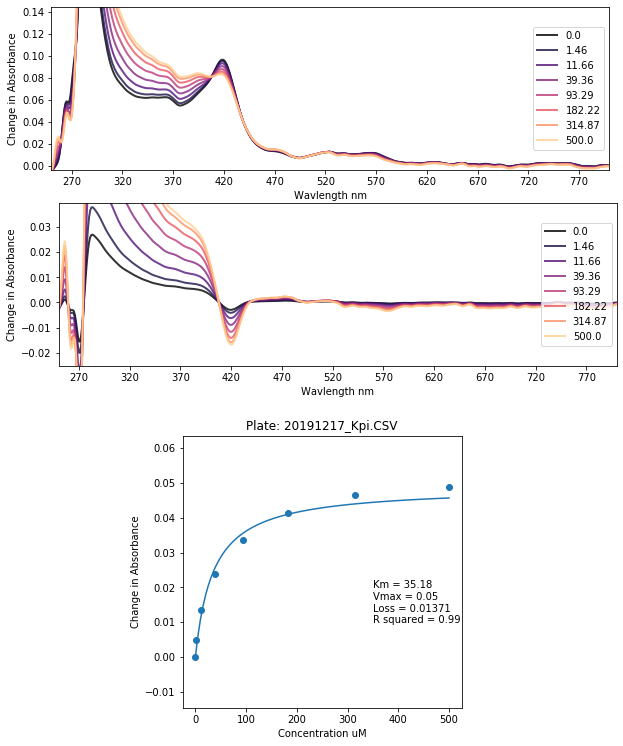
\includegraphics[width = \textwidth]{img/assay-dev-arachadionic.png}
\end{figure}

%%%%% -----------------------
\subsection{Assay Protocol} \label{protocol}

This is a assay protocol for detecting binding interactions between a Cytochrome P450 and multiple small molecule compounds.
The assay has demonstrated scale to a library of 980 compounds and five P450 mutants and with some small adjustments could be improved in scale and precision.

It works in 384 well microplates and uses a microplate reader to capture absorbance profiles from 220-800 nm wavelengths, from which a pattern associated with a P450-small molecule binding interactions can be detected and quantified.  

It was designed for profiling and modelling the effect of mutations on a P450's substrate binding preferences.
This was tested with five P450 mutants against 980 drug-like compounds.
It requires purified P450 protein which limits the rate of data generation, though can scale to more compounds.


\subsubsection{Requirements}

\textbf{Essential:}

\begin{itemize}
\item \textbf{Hardware:}
	\begin{itemize}
	\item \textbf{Microplate reader:} Able to read absorbance for all wavelengths between 220 and 800 nm.
		Used here: \textit{BMG ClarioStar and FluoStar} microplate readers.
	\item \textbf{Labcyte Echo [500 550]:} Acoustic liquid handlers for precise compound dispensing.
\item \textbf{Consumables:}
	In absence of a high precision liquid handling machine, serial dilution of compounds would probably be fine.
	\item \textbf{Enzyme:} A purified Cytochrome P450 - used here were mutants of P450 BM3 at ~800 µM. 
	Note that BM3 is fairly stable at room temperature which facilitates queuing large batches of plates to the plate reader.
	You could run the assay at a low temperature if you use a solvent other than DMSO, which freezes at 19ºC, which interferes with measurement.
	\item \textbf{Compound Library:} A large number of compounds in solvent (e.g. DMSO) in a microplate format.
	Used here was a 980 compound library, dissolved at 10 mM in DMSO in 96 well format.
	\item \textbf{Buffer:} must be optically clear the protein must be stable in it.
	Must not contain potential ligands.
	Used here was 100 mM Potassium Phosphate at pH 7.0 - chosen based on traditional wisdom.
	\item \textbf{384 well microplates - clear bottom:}
	Assay plates with at least 30 µl working volume. 
	Some treated surfaces may be more suitable for unstable proteins.
	Ideally have minimal absorbance in the 390-420 nm region, but this can be corrected for with controls.
	Used here: \textit{ThermoFisher Nunc 384 Well Plates}
	\item \textbf{384 well \textit{Labcyte Echo} source plates:} for dispensing compounds to assay plates. 
	Used here were the \textit{Low Dead Volume (LDV)} variety, which have a working volumne of 2.5-12.5 µl, 
	which limits compound waste compared to the standard \textit{Echo} plates (12-65 µl).
	\end{itemize}
\end{itemize}

\textbf{Optional:}
\begin{itemize}
	\item \textbf{Hardware:}
		\begin{itemize}
			\item \textbf{Bulk liquid dispensing:} can be far more accurate than a multichannel pipette when dispensing protein or buffer into wells.
			During development, both a \textit{ThermodropMulti} peristaltic dispenser and a \textit{Hamilton Star} liquid handling robot. 
			Both work well, though use of a bulk liquid dispensing machine is recommended given their speed, lower unit cost and lack of requirement for pipette tips.
			\item \textbf{Microplate reader plate loader:} Autoloading plates into the reader increases throughput capacity significantly.
			I used a \textbf{BMG ClarioStar} plate reader with a stacker module.
		\end{itemize}
	\item \textbf{Consumables:}
		\begin{itemize}
			\item \textbf{BSA:} in assay buffer may have a stabilizing effect on the enzyme - which would improve time stability and reduce errors.
			Time stability is important for scalability.
			\item \textbf{384 well Labcyte Echo DMSO Trays:} for control for DMSO concentration in assay wells by topping up each assay plate to a fixed concentration. 
			Around 5\% is ok with BM3.
		\end{itemize}
\end{itemize}

\subsubsection{Procedure}


\textbf{Summary:}
%\begin{enumerate}
%	\item \textbf{Design \textit{Echo} picklists}
%	\item \textbf{Dispense compounds into \textit{Echo} source plates}
%	\item \textbf{Dispense compounds from \textit{Echo} source plates to empty assay plates}
%	\item \textbf{Stopping point}
%	\item \textbf{Thaw purified P450 and make stock of ~ 10 µM in a neutral buffer, enough for 15.36+ ml per plate (40 µl per well)}
%	\item \textbf{Dispense the diluted protein into the assay plates, centrifuge etc}
%	\item \textbf{Capture UV-Visible light absorbance data between 220 and 800 nm from plates in a microplate reader at room temperature within 3 hours}
%	\item \textbf{Data analysis}
%\end{enumerate}



\begin{enumerate}
% --- 1---- 
	\item \textbf{Design \textit{Echo} picklists:}
	\begin{itemize}
		\item An \textit{Echo} can accept a \texttt{csv} file with column headers: \texttt{Transfer Volume}, \texttt{Volume}, \texttt{Destination Well}, \texttt{Source Well} and optionally: \texttt{Destination Plate Name} and \texttt{Source Plate Name}.
			The Volume must be in nano litres and a multiple of 2.5 and the Source and Destination wells must be in the format \texttt{[A-Z][0-9]+} and exist in the plate layout specified to the \textit{Echo} client at runtime.

		\item The picklist(s) can be generated in a spreadsheet exported to \texttt{.csv} or programmatically.
			Documentation for the \texttt{python} tools used are [documented here.](picklists.md)
	\end{itemize}
% --- 2---- 
\item \textbf{Dispense compounds into \textit{Echo} source plates}
	This can be done with a multichannel pipette, and requires one tip per compound. 
		If the total volume of each compound required is greater than 60 µl then a standard polypropylene \textit{Echo} plate should be used, otherwise a low dead volume plate may be economical
		If not, or for valuable compounds, Low Dead Volume \textit{Echo} may plates should be used.
		These have a working volume of 2.5-12.5 µl, outside of which the \textit{Echo} will refuse to dispense.
	You may need to dispense the same compounds into multiple source wells and the picklists must be designed accordingly.

% --- 3---- 
\item \textbf{Dispense compounds from \textit{Echo} source plates to empty assay plates}
		\begin{enumerate}
			\item Transfer the picklist \texttt{.csv} to the \textit{Echo} host computer.
			\item Launch the \textit{Echo Plate Reformat} client there:
			\item Create New Protocol 
			\item Select Custom Region Definitions
			\item \texttt{File} > \texttt{Import Regions} and select your picklist \texttt{.csv}
			\item \textbf{Optional:} Specify the log output in \texttt{Options}, simulate with \texttt{Run} > \texttt{Simulate} 
			\item Save and run, optionally simulating the run first. 
			Multiple copies of a set of destination plates can be specified if the source plates contain sufficient compound volume.
		\end{enumerate}

% --- 3---- 
	\item \textbf{Stopping point:} Length of pause depends on rate of DMSO evaporation from destination/assay plates and the stability of the compounds at the plate storage conditions. 
		Plates stored in a stack should limit evaporation rate to an extent, though specialised lids for \textit{Echo} plates that limit DMSO evaporation are available.
Up to 24 hours seems ok.
% --- 5---- 

\item \textbf{Thaw purified P450, make stock of ~ 10 µM in a neutral buffer, enough for 15.36+ ml per plate (40 µl per well)}
I heard that thawing fast limits ice crystal formation, which could destroy some protein.
Optionally, in a microcetrifuge, pre-cooled to 4C, spin the protein at 14,000 rpm and carefully transferr to fresh tubes to remove unfolded protein.
	\begin{enumerate}

	\item Measure the stock concentration of the protein in a UV-Vis spectrometer by taking an absorbance trace from 200-800 nm, diluted in the destination buffer.
	There should be a peak at 420 nm, the height of which can be used to calculate the protein concentration with the following equation:

			\begin{equation}
				[P450]  = a e l  
			\end{equation}

       where $a$ is absorbance and $e$ is the extiction coefficient - 95 for P450 BM3 heme domain.
       $l$ is the path length in cm and for the cuvettes used was 1.
       Use the measured stock concentration of P450 to create a working stock of around 10 µM.
       10µM was chosen because it yeilds a reasonably strong signal when in plates.
       Varying the protein concentration doesn't have a big effect on measurements, so err towards using more.


	\item Dilute in neutral buffer to the target working concentration.
	Filtration through a 22 µm syringe filter can remove some precipitates.
	Vacuum filtration can work too but in practice, the protein can pick up binding partners from the filtration equipment contaminants, which can ruin downstream measurements.
	\end{enumerate}

%!!! Warning
%	**Mixed Spin protein:** if the P450 is bound to a substrate it can squash the absorbance peak at 420 nm and raise a peak at 390 nm. 
%	This was an issue with BM3 mutants A82F and A82F/F87V which are particularly promiscuous.
%
%	![mixed spin spec]()
%
%	In this case, the substrate can be removed from the binding site using a column of a lipophilic resin, I used Lipidex 1000.
%	The resin is stored in methanol so it must be washed thoroughly with deionised water before equilibrating with the assay buffer.
%	Adding a salt-based buffer while methanol is still present can cause precipitation and block the column.
%
%	The thawed, mixed-spin P450 is added to the column and left at 4ºC for one hour.
%	It's advisable to create fresh stocks of assay buffer at this point, since it's possible that a buffer contaminant is the result of the mixed spin.
%	Then the protein is flushed from the column with more assay buffer into a clean bijoux and kept on ice.
%	Measure the light absorbance between 200 and 800 nm.
%	If the procedure was successful then the absorbance peak at 390 nm should have subsided and the peak at 420 nm should be high and useable for calculating the protein concentration.

\item \textbf{Dispense the diluted protein into the assay plates, centrifuge}

	An electric multichannel pipette works but accuracy is more limited than with automated dispensing. 
	38 µl of protein working stock needs to be dispensed into each well, which brings the total well volume to 40 µl in cases where the volume of compounds in DMSO in each well is 2 ul.
	If the volume of DMSO in destination wells is not a constant 2 ul, then default to 38 µl of the protein stock.
	The variation in total volume can be corrected for in compound concentration calculations, though the path lenght will vary which affects precision.

	Better than that is a precise bulk liquid handling device.
	I used a \textit{ThermodropMulti} for a while which was fast and accurate.
	Occasionally a nozzle would become blocked either with DMSO ice or precipitates, though the protein still dispensed into the correct well.
	Blockages can be cleared by disassembling the pump head, coupling a syringe of water to the nozzle and flushing.

	It may be necessary to dispense some control plates, with everything but protein.
	This is useful to correct for the intrinsic absorbance of the plate and buffer, as well as the compounds themselves which sometimes have absorbance at the measurement wavelengths.
	A control set of plates for every protein screen may be unnecessary and expensive. 
	One good one should be ok.

	Centrifuge the plates for 2-5 mins at around 2000 rpm to push the well contents to the bottom.
	This step can also ensure that meniscuses are flat and uniform and remove bubbles.
	If possible, centrifuge at room temperature to avoid DMSO ice formation.

\item \textbf{Capture UV-Visible light absorbance data between 220 and 800 nm from plates in a microplate reader at room temperature within 3 hours:}

	The protein is fairly stable over the course of 3 hours.
	On a BMG platereader, measurements take about 15 minutes per plate including the data transfer from device to host machine.
	Using an automated plate loader is recommended, for example a BMG Stacker module.
	In that case, put an empty or waste plate on the top of the stack to limit evaporation from the top assay plate.
	The BMG ClarioStar can be instructed not to read the last plate.

	The stacker occasionally jams due to a solenoid error, which can be due to a misaligned stack of plates.
	It is advisable to un-stack and re-stack the plates using the stacker to check for this kind of issue prior to measurement.

\item \textbf{Data analysis overview}
   \begin{enumerate}
	   \item Export the plate measurement data to a workable format, like \texttt{.csv}. 
	   In the BMG Mars software, the operation is simple but on all host machines I've tried it on have been unreasonably slow to open the data files prior to export.
   \item Index the files to their experiments. 
	   I used a \texttt{config.yml} file to track this.
   \item \textbf{Analysis}
		\begin{enumerate}
		\item Match compounds to plate well data.
		\item Match the \textit{Echo} exceptions report to wells to find the actual compound volume in each well.
		\item From each trace, subtract its own absorbance $A_{800}$ at 800 nm.
		   This accounts for baseline drift which can be caused by light scattering from precipitates.
		\item If correcting for compound absorbance with control plates, then subtract the absorbance of each test well from each control well.
		        If the actual compound volumes of the test and control don't match up, it can be an issue if the compound interferes with the absorbance in the 390-420 nm region.
		        If the compound absorbance changes predictably then it can be interpolated.
		\item Curves can be smoothed with Gaussian smoothing using \texttt{scipy.ndimage.gaussian\_filter1d} if necessary.
		        Sources of a jagged curve can be precipitates, which can interfere with downstream analysis.
		\item At this point, changes in the P450 absorbance trace can be identified.
		   Common categories of trace are:
			\begin{itemize}
			   \item Clean absorbance trace, no shift.
			   \item Clean absorbance trace, peak shift from 420 to 390 nm.
			   \item Clean absorbance trace, peak shift from 420 to 424 nm.
			   \item Compound interference in absorbance trace.
			   \item Light scattering in absorbance trace.
			\end{itemize}
		   \item For clean traces with a peak shift from 420 to 390 or 424 nm, biding response can be calculated using the $|\Delta A{390}| - |\Delta A_{420}|$ or $|\Delta A{420}| - |\Delta A_{420}|$  for each compound concentration.
		   With a set of concentration-response data points, the binding dissociation constant $K_d$ can be calculated using the Michaelis-Menten equation for enzyme kinetics:

				\begin{equation}
					Response = \frac{V_{max} \times [S]}{K_{d} + [S]}
				\end{equation}
				\begin{equation}
					Response = |\Delta A_{390}| - |\Delta A_{420}| 
				\end{equation}

		   Where $[S]$ is a given substrate concentration and $V_{max}$ is the maximum response magnitude possible from the P450 being tested from this compound.
				The metrics $K_d$ and $V_{max}$ can be derived by fitting $|\Delta A{390}| - |\Delta A_{420}|= \frac{V_{max} \times [S]}{K_{d} + [S]}$ can be fit to the P450 substrate concentration-response  data points using a curve fit algorithm like \texttt{scipy.optimize.curve\_fit}.

		   Useful additional metrics for each compound are $R^2$ score of the curve fit, a data quality metric. 

		   An ideal end output of this analysis as a table of compounds, P450s and a qualification or quantification of their binding interactions.

		\end{enumerate}
   \end{enumerate}
\end{enumerate}

\subsection{Enzyme Production}

\subsubsection{Summary}

This page contains the methods for producing the enzymes used in this screening program.
The enzymes are variants of the Cytochrome P450 BM3:

\begin{table}
	\begin{center}
		\caption{\label{bm3_table} BM3 mutants used in screening}
		\begin{tabular}{l|p{3cm}|l}
		\textbf{ID} & \textbf{Mutations} & \textbf{PDB} \\
		\hline 
		WT   &           & 1BU7 \\
		A82F &   A82F    & 4KEW \\
		DM   & A82F/F87V & 4KEY \\
		1YQO &   T268A   & 1YQO \\
		1YQP &   T268N   & 1YQP \\
		\end{tabular}
	\end{center}
\end{table}

The page shows the method used to create the mutant BM3 expression plasmid DNA, 
expression of the mutants in \textit{E. coli} and their purification.

\subsubsection{Aims}

\begin{itemize}
	\item Create expression plasmids containing the target mutants from an in-house starting point - \texttt{bm3-wt.gb}.
	\item Sequence the plasmids to confirm they carry the mutations
	\item Express the mutants in \textit{E. coli} using those plasmids.
	\item Purify the mutant protein from the \textit{E. coli} harvest.
\end{itemize}


\subsubsection{DNA}

\subsubsection{Starting Material}

An heirloom BM3 Wild-type (heme domain) expression plasmid, \texttt{bm3-wt.gb}, 
was inherited and used as the basis for DNA work in this project.
The plasmid is a pET14 expression vector where the BM3 gene has a 6xHis purification tag at the N-terminus,
flanked by a T7 promoter and terminator which leads to high yields in strains of \textit{E. coli} containing the T7 RNA polymerase.
The plasmid also encodes ampicillin resistance and a \textit{ColE1} replication origin which leads to a low copy number.


\subsubsection{Primer Design and Acquisition}

Mutations were introduced to the wild-type sequence via Polymerase Chain Reaction (PCR)-based site-directed mutagenesis.
Two methods were considered for this task based on commercially available kits, where each imposes different constraints on primer design.
Efforts were made to automate primer design as far as possible with scalability in mind.

The PCR kits used were:

\begin{enumerate}
	\item \textit{New England Biolabs (NEB) Q5 mutagenesis kit} - which requires that primers facilitate cloning of a linear DNA strand from the circular template plasmid and mutation payloads are carried in the tail of one primer.
	The kit includes a cocktail of the DNAse \textit{DPN1}, which disassembles template plasmid methylated in \textit{E. coli} and a kinase and ligase that work to join the ends of the linear DNA into a circular plasmid.
	The reaction is restricted to one payload.

	\item \textit{Agilent Quickchange mutagenesis kit} - which requires a pair of overlapping primers that carry the mutation payload in the mid-section.
	This cloning method produces circular DNA carrying the targeted changes. 
	It has the advantage of allowing multiple payloads carried by multiple primer sets.
\end{enumerate}

Two important considerations based on the template sequence are:

\begin{enumerate}
	\item Adenine-Thymine (AT) richness of the template sequence. Compared to cytosine and guanine (C and G), A and T bind to their complimentary bases weakly.
		This results in weak primer binding to the template sequence, measurable by a low primer \textit{melting temperature} $T_m$.
	To compensate, primers must be longer than they otherwise would be for a sequence richer in CG, which increases their cost and their chance of self-binding.
	The template sequence used here is AT-rich - at 42\%.
	\item Repetitions and palindromic regions of the template sequence. 
		If the sequence surrounding a mutation target area contains these features, then the likelihood of \textit{mis-priming} by binding to an off-target sequence area is high, so too is the likelihood of a non-functional, self-binding primer.
\end{enumerate}

\textbf{note: talk about \texttt{mxn}}

\subsubsection{PCR and Work Up}




\subsubsection{Sequencing}

Purified plasmid DNA ostensibly conataining the target mutations, having been harvested and purified from DH5a \textit{E. coli} cells, was shipped to \textit{Eurofins Genomics} for sequencing using their \textit{TubeSeq} service, which uses a variant of Sanger Sequencing.
Sequencing primers for this matched the T7 promoter and terminator and provided coverage of the targetted region.

\textbf{note: include sequencing, flesh out}


\subsection{Protein Expression}

Having been sequenced and confirmed to carry the target mutations, the mutant plasmids were used to produce the mutant protein \textit{en masse} via a \textit{BL21 DE3 E. coli} strain, which contains a T7 RNA polymerase under the control of a \textit{lac} promoter.
\par
BM3 mutants were expressed in \textit{NEB} BL21 (DE3) \textit{E. coli} cells grown in \textit{Formedium} auto-induction TB media at 25°C for 24 hours with shaking at 180 rpm. Cells were harvested by centrifugation in a \textit{Beckman} JA16 rotor at 6000 rpm for 10 minutes and stored at -20 °C. Variants were purified from the cells by nickel-affinity chromatography, dialysis into buffer 1, concentration to 500-1000 µM and storage at -80 °C. % protein prep

\subsubsection{Materials}

\begin{itemize}
	\item Expression plasmid encoding mutant P450 BM3
	\item \textit{BL21 DE3 E. coli} - NEB. This domesticated \textit{E.coli} strain is shipped in a transformation buffer.
	\item Auto-induction \textit{Terrific Broth} (TB) media, which contains glucose and a lactose analog. 
	The lactose analog triggers expression of T7 RNA-polymerase in \textit{BL21 DE3 E. coli} and the subsequent expression of the target protein between the T7 promoter and terminator regions. 
	The glucose inhibits this until it is consumed by the cells, which allows them to multiply to sufficient numbers before diverting energy to production of the target protein.
	\item Ampicillin - the antibiotic for which resistance is encoded in the target plasmid, ensuring that all cells in the growth media contain this resistance.
	Assuming no ampicillin-resistant contaminants, all cells should be \textit{BL21 DE3 E. coli} containing the target plasmid.
	\item $\Delta$ Amino-Levulnic acid ($\Delta$-ALA) - a precursor to heme, ensuring heme availability for the large amount of BM3.
\end{itemize}

\subsubsection{Method}

\subsubsection{Purification}

\subsection{Screening}

Throughput the screening process, the protocol described in section \ref{protocol} was employed.
Six concentrations of each target compound were dispensed with the aim of determination of the $V_{max}$ and $K_d$: 0.0, 5.26, 55.61, 156.72, 306.74 and 500 µM.
These values were generated from six linearly spaced values between 0 and 1 squared, then scaled to the starting concentration and final volume.
This method saved some compound compared to a straightforward linear spacing of values between 0 and 500 µM - the maximum concentration possible given a 10 mM starting stock in DMSO without exceeding a total of 5\% v/v solvent.
\par
During the first run, control experiments where compounds were present in buffer only were included for downstream correction of the compounds inherent UV-Visible light absorbance, though it was thought to be unnecessary to repeat this for each subsequent screen, since it is wasteful of resources, particularly the compounds themselves.

Each of the five enzymes was screened against all 980 compounds over the course of a day each.



% -------------------------------

\subsection{Model Design and Construction}

The model aims to predict the binding likelihood between a given protein sequence and chemical structure, illustrated in equation \ref{pbinding}.


\label{pbinding}
\begin{equation}
P_{binding} = fn(sequence, smiles)
\end{equation}


This page describes the deep learning model constructed for this project.
The model is designed to estimate the likelihood of a binding interaction between a given Cytochrome P450 sequence and a ligand SMILES code.
The intended end uses of the model are:

\begin{enumerate}
	\item Virtually screening sequences for potential activity with a given compound.
	\item Optimally design an enzyme-ligand screening experiment.
\end{enumerate}


\subsubsection{Approach: Recommender Systems}

Abstractly, the problem of predicting the binding likelihood between a one of $m$ proteins and one of $n$ small molecules can be likened to filling empty the values of an $n \times m$ matrix, where rows and columns refer to proteins and small molecules and values are the probability of a binding interaction between the two:

\begin{center}
$
\begin{matrix} 
	 & compound_i & compound_{i+1} & ... & compound_{i+n} \\
	sequence_i  & P_{binding_{i,j}} &  &  & \\  
	sequence_{i+1} &  &  &  &  \\
	 \vdots &  &  & \ddots &  \\
	sequence_{i+m} &  &  &  &   \\
\end{matrix}
$
\end{center}

Some $P_{binding}$ values are known, which in the perspective of $n \times m$ possible values where $n$ and $m$ approach infinity, coverage is sparse.

This type of problem has been addressed in recommender systems, which in the context of streaming services translates to a matrix of $n$ users and $m$ paces of content.
Known values are likes and engagement metrics and are similarly sparse, and blanks can be filled with the probability of a successful recommendation.

Machine learning models can be trained to predict the unknown values based on a numerical representation of the user and content.
The prediction can be cast as a classification problem.
To overcome the lack of negative data points, presumed negative data can be generated by sampling a random user: content pair, which should be treated with caution.

In this work, a machine learning model classifies pairs of protein sequence and small molecules as binding or not.
Negative samples are generated by randomly sampling a sequence and small molecule, which given the vastness of sequence and chemical space may be reasonable in a large number of cases, though this assumption is treated with caution.
A Binary Cross Entropy loss function is employed here where true positives and synthesized negatives are weighted evenly.

\subsubsection{Data}

Small molecules are represented as SMILES codes in the dataset, which are parsed using \texttt{rdkit} and then into 2048 bit fingerprint vectors using the \texttt{RdkitFingerprint}.
Molecular fingerprints are generated by hashing functions based on an input molecule such that similar molecules are assigned similar fingerprints, which makes them useful in featurizing small molecules for machine learning tasks.
The fingerprints are represented as a $b \times 2048$ tensor where $b$ is batch size.

Sequences are represented in the dataset as strings where each character $c_i$ is a single letter amino acid code:

$$
c_i \subset{ACDEFGHIKLMNPQRSTVWY}
$$

Roughly, characters are encoded as tensors of the integers that index their position in the list $\begin{matrix} ACDEFGHIKLMNPQRSTVWY\end{matrix}$, with extra positions to represent null values, start of frame and end of frame characters.

\subsubsection{Pre-Training Data}

A dataset of around $10^6$ protein sequences and SMILES codes for their corresponding binding partners are gathered here from several sources.

There are several sources of data containing protein sequences and information on their binding partners.

\begin{itemize}
	\item \href{https://www.uniprot.org/}{Uniprot} is a large, publicly available database containing protein sequences and a variety of functional annotations. 
		\textit{Uniprot} comprises three databases:
	\item \textit{UniProt Knowledgebase (UniprotKB)} contains protein sequences and their annotations.
		\textit{UniprotKB} mainly comprises two collections:
\item \textit{SProt:} - The SwissProt collection. Manually annotated and non-redundant protein sequences. 
	Annotations can include \textit{Enzyme Comission (EC)} classification numbers, which can be linked to substrates and products. 
		At the time of collection (2022) the \textit{SProt} collection contains 1,706,449 data points.
	\item \textit{Trembl:} - The TrEMBL collection. Automatic annotations, N data points.
	\item \textit{UniProt Archive (UniParc)} - an archive of sequences pooled from other public protein sequence databases.
	This collection does not contain annotations.
\item \textit{UniProt Reference Clusters (UniRef)} - Three collections of clustered sequences from \textit{UniprotKB} and \textit{UniParc}. 
	Each collection is clustered with the CD-HIT algorithm and a different similarity cutoff: \textit{UniRef100}, \textit{UniRef90} and \textit{UniRef50} use 100, 90 and 50\% respectively.
	In the case of UniRef100, similarity measurements are made against sequence fragments.
	The clusters do not contain annotations.
		Importantly: \textit{Uniprot} files can be freely downloaded via an \texttt{ftp} server at \href{https://ftp.uniprot.org/pub/databases/uniprot/current_release/uniref/}{https://ftp.uniprot.org/pub/databases/uniprot/current\_release/uniref/}
	\item \href{https://www.genome.jp/kegg/}{KEGG} is another large source of proteins and biological function annotations, though download of the full dataset is restricted to paying customers.
		\textit{KEGG} does however have a \textit{REST API} which can be used to query the database, though requests are handled somewhat slowly.
		Despite this limitation, it was useful to cross-reference \textit{EC} numbers against substrate and product identities.
	\item \href{https://www.bindingdb.org/bind/index.jsp}{BindingDB} is a large collection of proteins and known small molecule binding partners mostly derived from high throughput drug screening datasets, which is reflected in the chemical diversity of the set.
	\item \href{http://pdbbind.org.cn/}{PDBBind} contains protein sequences and structures and their binding ligands derived from the \textit{Protein DataBank (PDB)}.
	\item \href{https://www.brenda-enzymes.org/}{BRENDA} contains manual curations from primary literature for enzymes.
\end{itemize}


For this work, the Uniprot SProt and BindingDB collections were selected because they met the necessary requirements of containing protein sequences that can be matched to a chemical binding partner.
For data mining a cloud machine was hired (Linode \texttt{g6-dedicated-8}, 1TB Disk space, 8 \texttt{x86\_64} cpus, 16 GB RAM, Debian 10, New Jerse
Scripts used here are in \texttt{screening-fist/data/pretraining/scripts/}.

Large files and files in large numbers can prove slow to search, a problem that databases address.
For this work, a database was set up on the hired machine for storage and retrieval of the mined data.
MongoDB, an unstructured database, was chosen. 

MongoDB is unstructured in as far as it does not store tabular data, instead opting for a \texttt{json}-like schema which uses attribute:value arrays that themselves can contain more attribute:value arrays.
This offers considerable flexibility in data input from heterogeneous sources with varying presence, absence and categories of annotation.

SProt was gathered as a compressed \texttt{.dat} file using \texttt{screening-fist/data/pretraining/scripts/uniprot.sh}, which decompresses, parses entries and uploads them to the local MongoDB in a single UNIX pipe.
Using a single pipe saves the need to store the decompressed file on disk, which becomes significant in the case of the \texttt{TrEMBL} collection which has an uncompressed size of around 700GB as opposed to the 3.5GB of \texttt{sprot}.

BRENDA was used for its comprehensive list of EC numbers which would later be used for reference.
BindingDB was downloaded in full as a \texttt{.tsv} file.
Both the BRENDA and BindingDB sets were downloaded using \texttt{curl} commands and BindingDB was uploaded to the MongoDB instance.

The EC numbers from BRENDA were used with the KEGG REST API to collection compound identification numbers, which in turn were used to retrieve SMILES codes from PubChem using the script \texttt{ec.py}
\texttt{mkdataset1.py} was used to assemble a \texttt{csv} containing protein sequences and SMILES codes of their binding partners (1,587,674), which was further filtered to exclude SMILES codes and sequences that could not be parsed using RDKit and the tokenizer used in the sequence model.

Finally, an attempt to improve the chemical diversity of the pre-training dataset was made.
A diversity filter that aims to return a subset of a compound set by maximizing the pairwise Tanimoto similarity of the subset compound fingerprints was employed using the MaxMin algorithm.


Unfortunately, MaxMin is $O(n^2)$ complexity, so is only feasible with relatively small batches.
64 compounds are selected this way from each batch of 512 from the filtered set, yielding \texttt{o3.csv} (1359834 data points and 908M uncompressed size).

\texttt{o3.csv} was compressed with \texttt{gzip} and loaded to an area of \textit{Linode} object storage in Frankfurt, making it accessible to the \textit{Linode} instances that would be used for model training.

\texttt{o3.csv} contained at least one invalid SMILES or sequences which had the costly effect of crashing the first model training run.
A filter for troublesome inputs was built and yeilded \texttt{o3f.csv} (826 MB).
and
For the purposes of model training and evaluation, the \texttt{o3f.csv} dataset was split 3:1 into a training and test datasets  \texttt{o3f.train.csv} and \texttt{o3f.test.csv} of sizes 907214 and 226804 respectively.


\subsubsection{Training Data}

\subsubsection{Model Architecture}

Given the model aims to predict:
$$
P_{binding} = fn(sequence, smiles)
$$

A neural network was devised to generate a prediction of $P_{binding}$ from an input of a protein sequence and a chemical SMILES code.
The network can be split into three parts:

\begin{itemize}
	\item \textbf{Sequence Embedding:} For a given protein $sequence$, output a tensor encoding a neural embedding $z_{sequence}$.
	\item \textbf{Chemical Embedding:} For a given chemical $smiles$ encoding, outputs an embedding $z_{smiles}$.
	\item \textbf{Prediction Head:} For the embeddings $z_{smiles}$ and $z_{sequence}$, output a prediction $P_{binding}$.
\end{itemize}

The architecture is illustrated in \ref{modelarch}.

\begin{figure}
	\begin{center}
	\caption{\label{modelarch} Architecture of the model constructed for this project}
	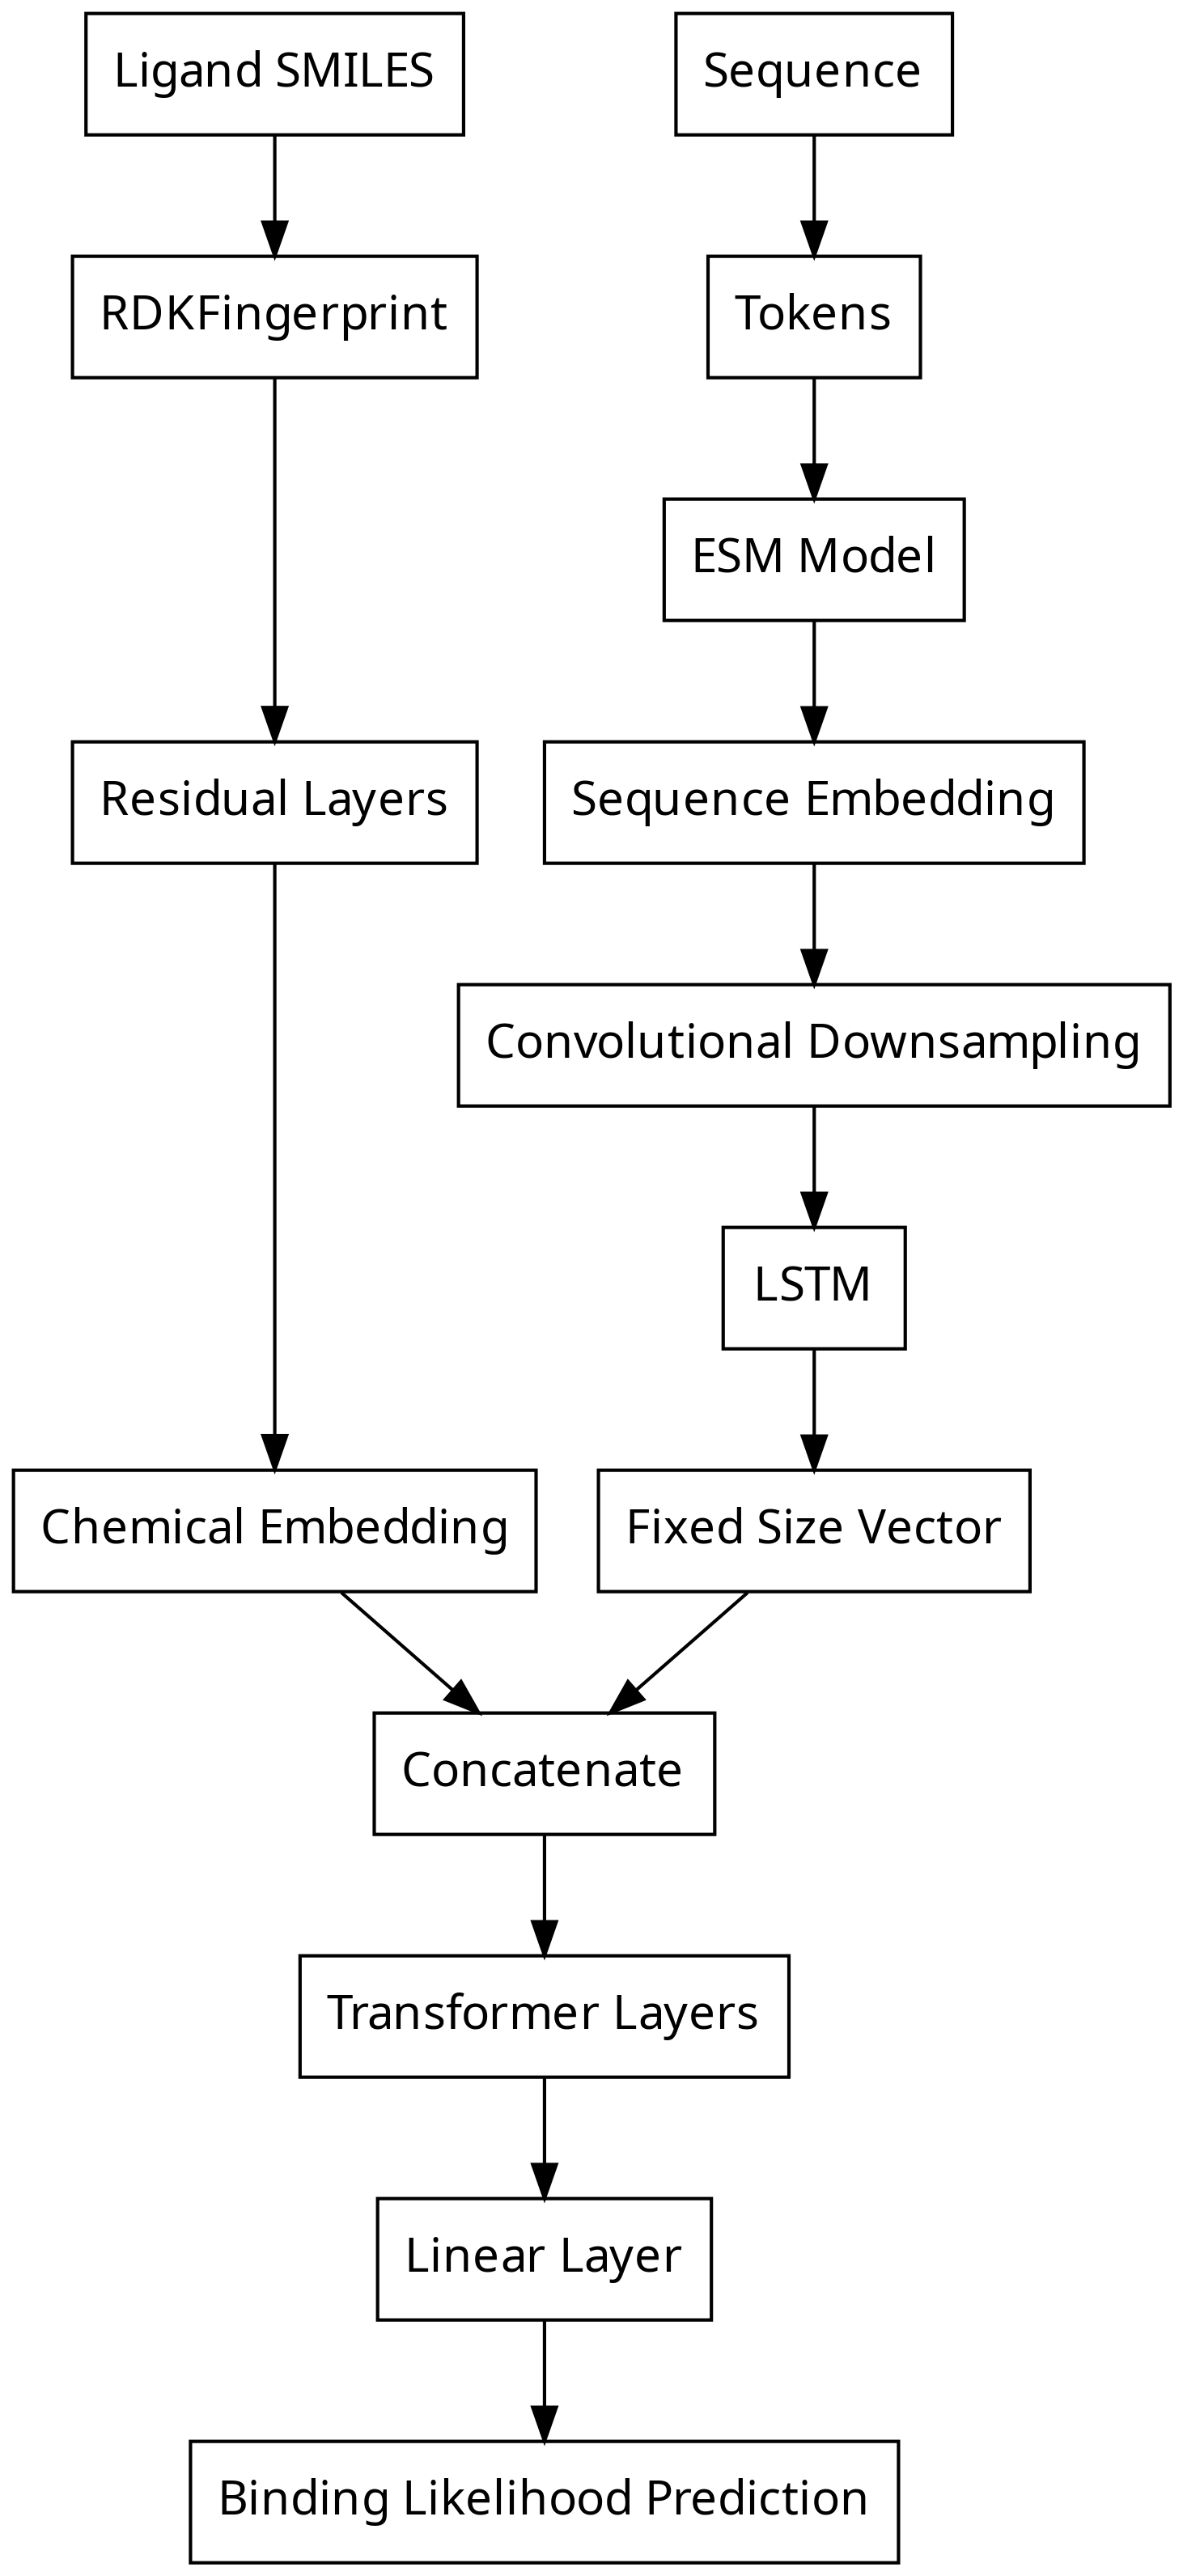
\includegraphics[height=0.8\textheight]{img/model.png}
	\end{center}
\end{figure}

\subsubsection{Sequence Embedding}

%Sequences were embedded using the pre-trained \texttt{esm1_t6_4equation 3M_UR50S} model \cite{rives2021biological}, which receives an input of a tokenized protein sequence and outputs a tensor of size $b l d$ where $b$ is batch size, $l$ is sequence length and $d$ is 35.

Although this model is the smallest of the ESM collection, on the single \textit{NVIDIA Quadro RTX 6000} used it still occupied most of the 24 GB of available memory and most of the processing capability, which lead to long training times and difficulty in training more than one model in parallel on the same machine.

This could be remedied, however since in the complete \texttt{o3f.csv} dataset and the screening dataset there are 2947 unique sequences, so it was economical to pre-compute the embeddings and save them to disk.
This resulted in a roughly 4$\times$ speedup in training time and massively reduced the memory requirements, allowing several models to be trained in parallel on a single GPU.
This also saved costs significantly.

\subsubsection{Chemical Embedding}

As mentioned, chemical SMILES were hashed into chemical fingerprints using the \texttt{rdkit} \texttt{RDKFingerprint} method as a means of representation, yielding a 2048-bit vector for each compoundagainThe vectors were converted to tensors and served as an input to a residual neural network that output an embedding that would later be used to form a combined representation of both compound and sequence for binding likelihood prediction.

\subsubsection{Prediction Head}

The combined sequence and compound embeddings served as input to the prediction head, which output a single number that indicated a binding likelihood prediction for the two inputs.

Both residual neural networks and transformers were compared as prediction head architectures.
Each consisted of 2-6 stacked layers of either residual or transformer layers with a fixed hidden layer size for convenience of automated assembly.
The final layer in both cases was a single linear layer with a single output and a sigmoid function to output a number between 0 and 1 representing binding probability.

\subsubsection{Pre-Training, Training and Evaluation}

Training was done in two stages, each with a performance evaluation, during which several models with varying architectures and hyper-parameters were trained and compared.
All training was done on a \textit{Linode} \texttt{g1-gpu-rtx6000-1} in New Jersey which cost \$1.50 per hour and was equipped with hardware specifications described in \textbf{table \ref{hardwaretable}}.

\begin{table}
	\begin{center}
		\caption{\label{hardwaretable} Hardware specifications for machine used in model training.}
		\begin{tabular}{l|p{3cm}|l|l}
			\textbf{Item} & \textbf{Specifications} & \textbf{Number}  & \textbf{Size}\\
		\hline 
		CPU  & Intel(R) Xeon(R) Gold 6148 CPU @ 2.40GHz & 8 \\
		RAM  & ?  & N/A & 30 GB \\
		Disk & ?  & 1   & 630 GB \\
		GPU  & NVIDIA Quadro RTX 6000 & 1 & 20 GB VRAM \\ 

	\end{tabular}
	\end{center}
\end{table}

\begin{enumerate}
	\item \textbf{Pre-Training:} This was done with the larger, more general \texttt{o3f} dataset, which was randomly split into training and validation partitions, the latter of which was used sparingly to avoid model bias.
	Pre-training lasted up to 64 epochs with a batch size up to 64.
	For each sample, a random sequence and SMILES pair were sampled as a presumed negative sample.
	The loss function used was binary cross entropy used with an Adam (Adaptive momentum) optimizer.
		Loss was tracked live using the \textit{Weights and Biases} API which was useful to evaluate models as they trained and terminate them where necessary.
	Model weights were saved in each epoch and after training the model was evaluated for precision and accuracy on a subset of the training data.
	The metrics gathered were: 

		\begin{enumerate}
			\item Mean binary cross entropy loss over evaluation.
			\item Mean precision
			\item A confusion matrix
			\item A receiver operator curve (ROC)
			\item A precision recall curve
			\item A detection error trade-off (DET) curve
		\end{enumerate}

	\item \textbf{Training:} This was done with the manually annotated screening dataset.
	An issue with the data was the class imbalance in that there were very few positive examples relative to negative.
		This was addressed by using \textit{Synthetic Minority Oversampling} (SMOTE) whereby the rarer positive data were re-sampled until they number that of the negative data.
	The total size of the re-sampled data was 6666 points, which were then split 3:1 into training and validation sets of size 4999 and 1667 respectively.
		A model pre-trained on the larger \texttt{o3f} dataset was re-trained on this set and evaluated for performance in the same manner as with the \texttt{o3f} data, visualised in the following section.
\end{enumerate}

\subsubsection{Evaluation}

%## Sequence Optimization
%
%## Active Learning


% ----------
\section{Results}
\subsection{Screening Data Analysis}

The data gathered for the screening experiments was saved in the \texttt{git} repository  \texttt{https://github.com/jamesengleback/screening-fist} in the \texttt{lab} directory.
Within the \texttt{lab} directory are directories for each screening experiment.
These include a \texttt{config.yml} file which maps data files to experiments for analysis.
\par
The script \texttt{sxfst/scripts/data\_proc2.py} was used to process the data into a large \texttt{csv} file containing each raw trace and its metadata.
By consolidating the data into a single file, fewer time-consuming operating system calls are made in downstream analysis which decreases the time cost of those tasks.

The script attempted to use the \textit{Echo} logs from each run to calculate the actual volume of each compound dispensed, since towards the end of the screening program shortages of compound made it impossible to fully dispense some experiments.
In retrospective this function did not perform properly, since all experiments are later annotated as having the target volumes of each compound.
This cannot be the case since it was casually observed that some compounds were completely depleted by the end of the screening program.
This issue is significant, leading to false negatives where a lack of response cannot be attributed to either a lack of compound or a true negative response.
This coding issue can be solved, but was not due to time constraints.

The downstream analysis in question was done using the script \texttt{sxfst/scripts/data\_analysis.py} which normalizes the traces, subtracts the control traces from them and calculates the P450 response to each compound, creating a plot in the process.
An example of one such plot is in \textbf{figure \ref{screeninghit}}.

The traditional response calculation method using $\Delta A_{390} - \Delta A_{420}$ proved ineffective for analysis of this data due to the noise, which would often result in scattering that increased the absorbance at the short wavelengths in ways that were occasionally unpredictable.

Instead, the gradient of each trace was taken by convolution of the kernel $\begin{bmatrix} -1 & 0 & 1 \end{bmatrix}$ across the smoothed and normalized traces.
The gradients were invariant to total absorbance, which was often perturbed by what appeared to be light scattering, but achieved a similar effect to calculation of $\Delta A_{390} - \Delta A_{420}$.
From the gradients, response was calculated as $|{\frac{\delta y}{\delta x_{390}}}| + |{\frac{\delta y}{\delta x_{420}}}|$.

Although this proved successful, the automated curve fitting to the response was not, outputting a constant value of 32 µM for each experiment - the lower $K_d$ bound.
With extra development this issue can likely be solved, but in order to keep within time constraints, an alternative solution was implemented.

%% manual annotation

The alternative solution was manual annotation of the plots output by the script.
Though crude, this method did yield a list of ostensible \textit{hits} as well as a list of anomalous results that were to be ignored.

Using this approach, 149 hits of the total 4900 compounds were identified, listed in the file \texttt{lab/hits.txt} in the repository.
These were used to create a \texttt{csv} file containing the full sequence and SMILES code for each enzyme compound pair and a boolean value that was true if that experiment was annotated as a \textit{hit}.
There are several drawbacks to this that should be noted:

\begin{itemize}
	\item \textbf{Human Error:} Although several passes over the data were done, the order was never randomized and there was only one annotator. 
		Since there are 4900 experiments, even if the annotator averages 1 second per annotation the runtime of an annotation run is 81 minutes, which will likely cause fatigue and subsequent errors.
		Since the order was not randomized, fatigue-induced error is more likely to occur in the same regions of the dataset in each pass.
	\item \textbf{False Negatives} due to a lack of properly functional compound concentration calculation, which would yield results that appear negative due to a lack of compound without being properly labelled as such.
		Another source of false negatives is the obfuscation of hits by noise in the traces due to scattering or compound absorbance that in some cases proved hard to correct for.
\end{itemize}

\begin{figure}
	\caption{\label{screeninghit} A good example of a positive result or \textit{hit} between BM3 A82F and \textit{Gestodene}. $K_d$ was calculated as 32 µM, which reflects an issue in the curve fitting rather than the actual $K_d$. \textbf{note - rescale axes, move kd text, legend title}}
	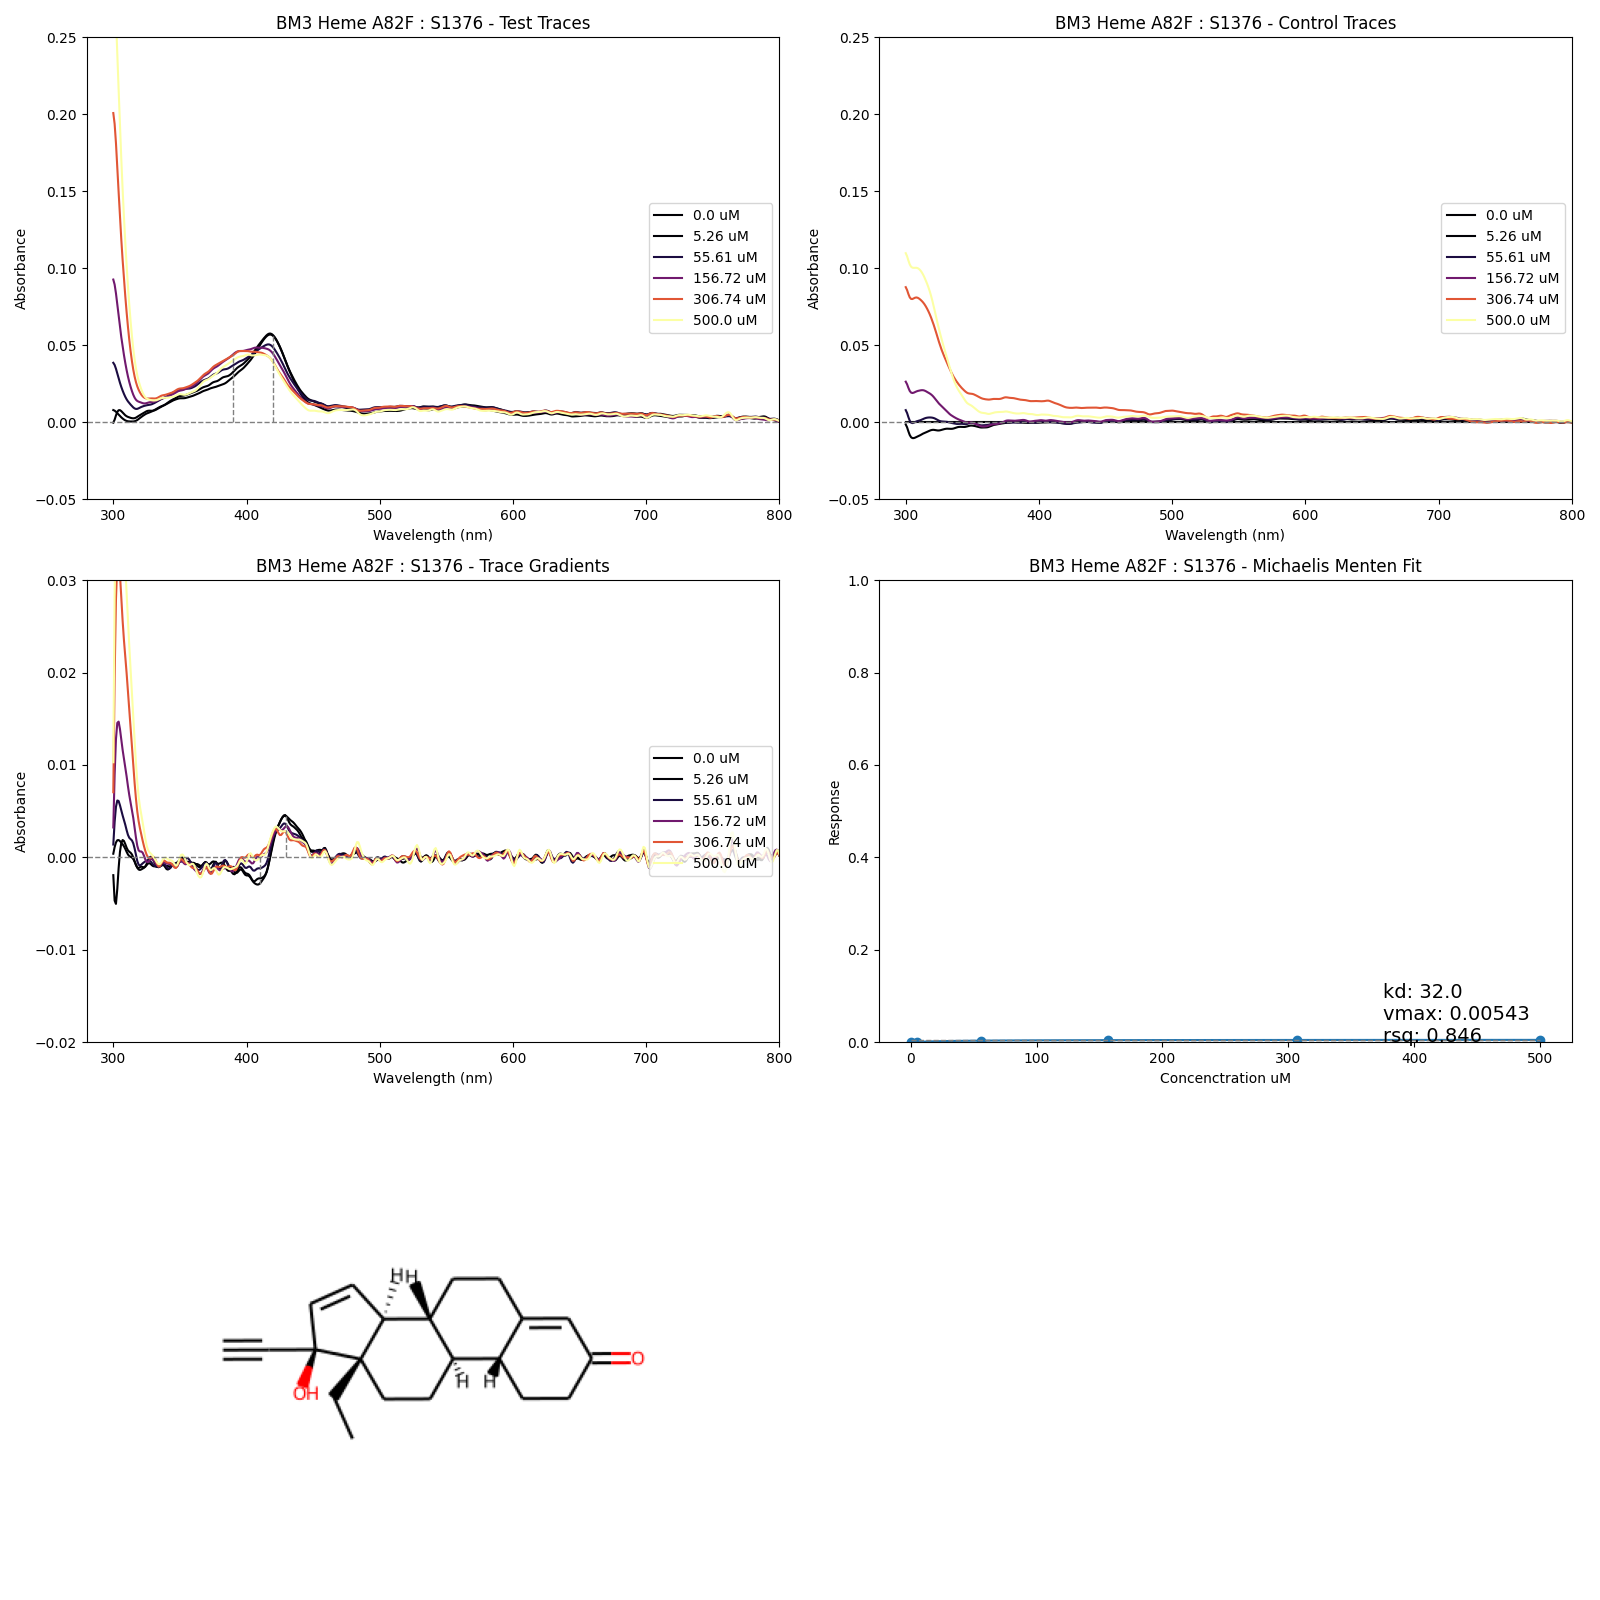
\includegraphics[width = \textwidth]{img/BM3-Heme-A82F:S1376.png}
\end{figure}

\subsection{Model Training}

\subsubsection{Pre-training}

Given constraints on money towards computing resources, a hyper-parameter sweep was not viable.
Instead, a small selection of models were trained and evaluated and the best of those was retrained on the screening data.
Model architecture and hyper-parameters were directly configurable by supply of arguments to the training script \texttt{model/train.py}, from which the best performing model was obtained using the command \texttt{./train.py -i data/o3f.train.csv --transformer --cuda --emb\_size\_head 2560 --n\_layers\_head 3 --emb\_size\_fp 512 --n\_layers\_fp 4 --num\_conv\_layers\_pool 3 --kernel\_size\_pool 9 --stride\_pool 3 --lstm\_hs\_pool 1024 --lr 1e-5 --batch\_size 64 -e 32
}, which is consolidated in \textbf{table \ref{frostybreezeparams}}.

\begin{table}
	\caption{\label{frostybreezeparams} Parameters for the best performing model in pre-training, designated the identifier \textit{frosty-breeze-83} by the \textit{Weights and Biases} API.}
	\begin{center}
	\begin{tabular}{ll}
		\textbf{Parameter} &     \textbf{Value} \\
		\hline
		lr                   &             $10^{-5}$ \\
		esm                  &   esm1\_t6\_43M\_UR50S \\
		cuda                 &                True \\
		load                 &                None \\
		test                 &               False \\
		input                &  data/o3f.train.csv \\
		epochs               &                320 \\
		batch\_size           &                640 \\
		emb\_size\_fp          &               512 \\
		n\_layers\_fp          &                 4 \\
		stride\_pool          &                 3 \\
		transformer          &                True \\
		lstm\_hs\_pool         &              1024 \\
		emb\_size\_head        &              25 \\
		n\_layers\_head        &                 3 \\
		kernel\_size\_pool     &                 9 \\
		num\_conv\_layers\_pool &                 3 \\
		num\_lstm\_layers\_pool &                 2 \\
	\end{tabular}
	\end{center}
\end{table}

%img/frosty-breeze-83-eval.png
%img/frosty-breeze-83-vivid-breeze-91-devout-thunder-90-eval.png
%img/frosty-breeze-83-vivid-breeze-91-eval.png
\begin{figure}
	\caption{\label{frostybreeze} Model evaluation report after pre-training for the model designated \textit{frosty-breeze-83}. Evaluation was on \texttt{o3f.test.csv} - a held-back partition of the pre-training dataset. Depicted are:
	mean binary cross entropy loss the course of training on \texttt{o3f.train.csv},  
	a confusion matrix, 
	a receiver operator curve (ROC), 
	a precision recall curve,
	a detection error trade-off (DET) curve and 
	mean precision and mean binary cross-entropy loss over evaluation.}
	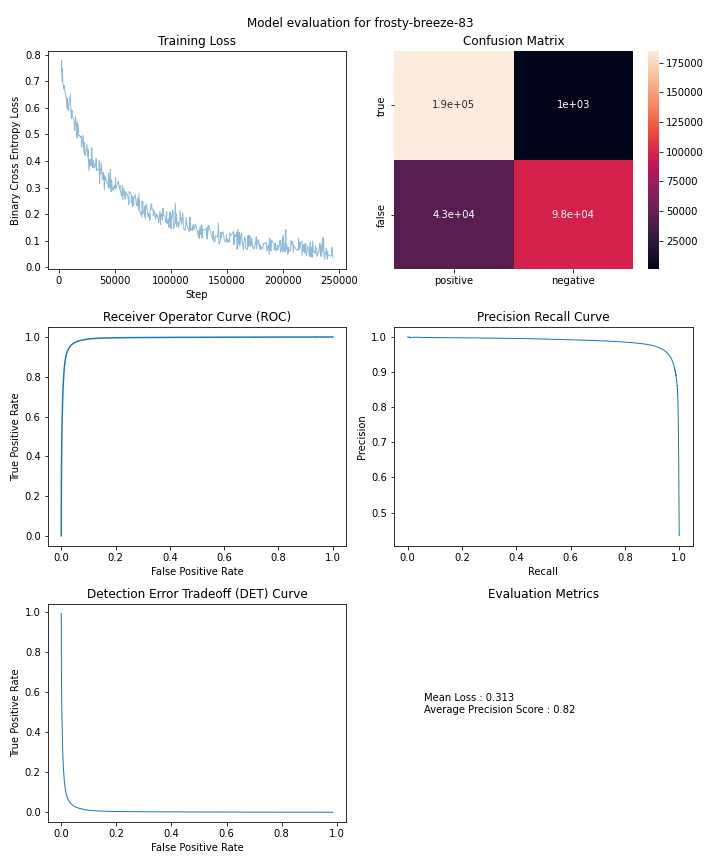
\includegraphics[width = \textwidth]{img/frosty-breeze-83-eval.png}
\end{figure}

\begin{figure}
	\caption{\label{devoutthunder} Model evaluation for another instance of \textit{frosty-breeze-81}, this time designated \textit{devout-thunder-90}, again retrained on the lab-based screening dataset \texttt{screening-data.train.csv} and evaluated on \texttt{screening-data.test.csv}. The report uses the same methods as in figure \ref{frostybreeze}}
	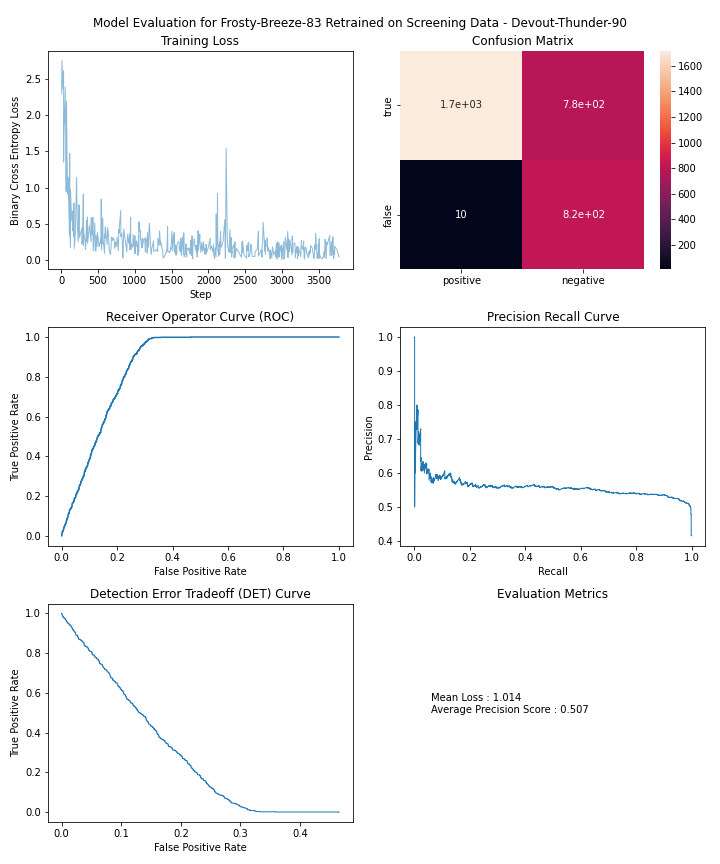
\includegraphics[width = \textwidth]{img/frosty-breeze-83-vivid-breeze-91-devout-thunder-90-eval.png}
\end{figure}
\begin{figure}
	\caption{\label{vividbreeze} Model evaluation report after pre-training for the model designated \textit{vivid-breeze-91}.}
	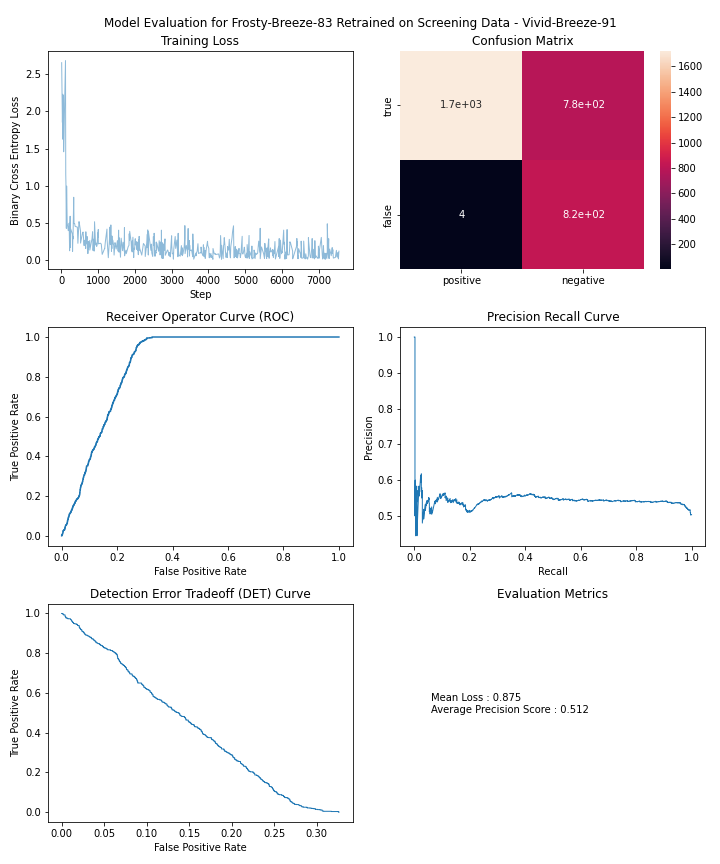
\includegraphics[width = \textwidth]{img/frosty-breeze-83-vivid-breeze-91-eval.png}
\end{figure}
\subsection{Model Application}
% ----------
\section{Discussion and Future Work}

\begin{itemize}
	\item \textbf{Improvements (Issues):}
	\begin{itemize}
		\item \textbf{Issues with screening library}
		\item \textbf{Improvements to data processing - recover compound concentrations}
		\item \textbf{Improvements to screening dataset partitioning}
		\item \textbf{Improvements to model application}
	\end{itemize}
\end{itemize}

\printbibliography

\chapter{Virtual Directed Evolution}
\section{Abstract}
% ----------------
\section{Introduction}

\subsection{Background}
\subsubsection{Herbicide Resistant Crops}
Herbicide-resistant crops are important for global agriculture because they mitigate yield losses due to weeds and give farmers extra flexibility in their herbicide application programs, which is important to suppress emergence of herbicide-resistant weeds. 
% value statement

Herbicides kill plants by inhibiting key metabolic processes and their species-specificity is determined by susceptibility of herbicide target and their ability to  metabolize the herbicide. % herbicide overview
HPPD inhibitors are a key herbicide class that cause leaf bleaching and death in susceptible plants. 
HPPD inhibition  disrupts tyrosine catabolism which disrupts UV-protection via carotenoid production and photosynthetic electron shuttling via plastoquinone, leading to death by UV damage and radical toxicity. % HPPDs

Engineering HPPD-inhibitor resistance into plants have used the HPPD and metabolic enzymes from naturally resistant species like \textit{Avena fatua}, which employs cytochrome P450 Cyp72A1  to initiate metabolism of mesotrione by ring hydroxylation at $C_5$.
In this case, the $C_5$ hydroxylation acts as a target site for glutathione-S-transferases which conjugate glutathione to xenobiotics.
The glutathione conjugate tags the xenobiotic for sequestration in the cell vacuole, which neutralises the threat.

Engineered Cyp72A1 has been explored as a means of HPPD herbicide in soybean, which is an important target recipient for HPPD resistance traits. % cyp 72a1 & engineering attempts
%%%%% CYP71A1 stuff

\begin{figure}
	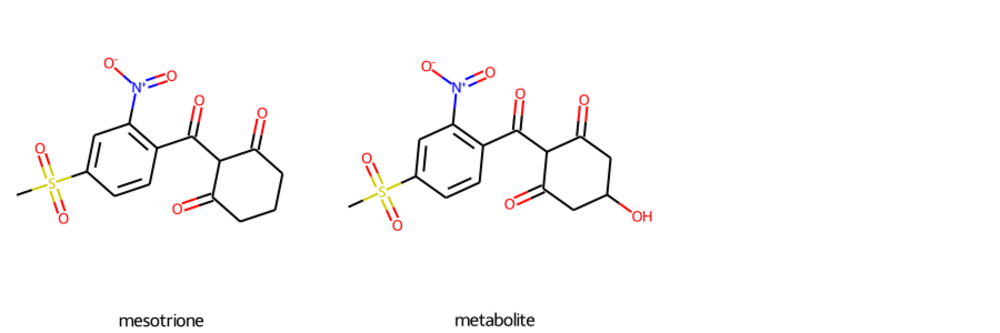
\includegraphics[width=\textwidth]{img/mesotrione+metabolite.png}
	\caption{\label{mesotrione} The HPPD inhibiting herbicide mesotrione and its primary metabolite 5-hydroxy-mesotrione in resistant strains of \textit{A. fatua}.}
\end{figure}

\subsubsection{Cytochrome P450s}
Cytochrome P450s are a ubiquitous class of heme-dependent oxido-reductases that are frequently involved in xenobiotic metabolism. % P450s overview
Bacterial P450s have been engineered to catalyse a range of xenobiotic biotransformations. 
The bacterial P450 BM3 from \textit{Bacillus megaterium} is one such bacterial P450 whose structure has been studied extensively. 
The A82F/F87V mutant has a broad substrate specificity, however it has no activity towards the HPPD herbicide mesotrione. % bacterial P450 engineering

\subsubsection{Virtual Directed Evolution}
Enzymes can be designed computationally using a genetic algorithm that evaluates the fitness of mutants by simulating the interaction between a target substrate and the predicted structure of the mutant. % computational enzyme edsign

The structure of a mutant can be predicted based on a template using techniques such as side-chain repacking by stochastic sampling from rotamer libraries and loop remodelling by cyclic coordinate descent. % structure pred - side chain repacking and loop ccd

% vde
Binding site interaction can be predicted using molecular docking, which attempts to predict likely protein-ligand binding conformations. 
A combination of the energy score and the conformation of docked molecules can be used to estimate likelihood of desirable reaction and therefore the fitness of a mutant. %score
In rounds of selection within a genetic algorithm, the fitness of a batch of mutants is evaluated by scoring desirability of protein-ligand binding, the fittest mutants are selected for breeding, in which mutants have elements of their genes recombined are further mutated, then the cycle repeats.   % genetic algorithms

\subsection{Technologies Used}
\subsubsection{Directed Evolution}
\subsubsection{Structure-Based Design}
\subsubsection{Protein Structure Prediction}
\subsubsection{Docking}
\subsubsection{Sequence Optimization Algorithms}
\subsubsection{Overview of this work}
\subsubsection{Engineering Problem}
\subsection{Overview of this Work}

Here, in attempt to engineer a mutant of the Cytochrome P450 BM3 to hydroxylate mesotrione at the $C_5$ position is made by developing a \textit{VDE} system, deploying it at scale on cloud infrastructure and identification on clusters of putatively active mutants.
% ----------------
\section{Methods}

The project was operated as a  \texttt{git} repository which can be found at:

\href{https://github.com/jamesengleback/vde}{https://github.com/jamesengleback/vde}.
The structure of the directory is:

\begin{itemize}
	\item \textbf{docs/:} write up for this document and markdown documentation
	\item \textbf{nb/:} jupyter notebooks used for data analysis
	\item \textbf{scripts/:} scripts to create and configure cloud machines to run algorithm on
	\item \textbf{vde/:} the vde algorithm configured to optimize BM3 for desirable mesotrione binding
\end{itemize}

This section details the implementation of this project:
\begin{itemize}
	\item The project is dependent on a \texttt{python} package \texttt{enz}, developed here for protein structure prediction and molecular docking to predict the behaviour of mutants; described in \ref{enz}.
	\item A score function that attempts to predict the likelihood of a $C_5$ hydroxylation of mesotrione is described in section \ref{scorefn}.
	\item A genetic algorithm to optimize the sequence of BM3 mutants is discussed in section \ref{ga} 
	\item Section \ref{cloud} describes execution of the algorithm at scale on cloud infrastructure.
\end{itemize}


% ---------------- enz ---------------- 
\subsection{\texttt{enz} \label{enz}}

Abstraction and modularization of protein structure prediction and molecular docking was important for reducing complexity of experiments and developability of the algorithm.
To this end the \texttt{python} package \texttt{enz} was created, an \textit{Application Program Interface (API)} wrapper around the \textit{PyRosetta} \cite{chaudhury2010pyrosetta} protein structure prediction software and the \textit{Autodock VINA} \cite{trott2010autodock} binary, as well as utilities to handle file format conversion using \textit{OpenBabel} \cite{o2011open}.
The package is modular enough to allow replacement of its functionality-providing back-ends according to a users requirements and is hosted at \href{https://github.com/jamesengleback/enz}{https://github.com/jamesengleback/enz}.

\texttt{enz} performs the following functions:
\begin{itemize}
	\item \textbf{Protein Structure Prediction:} \texttt{enz} uses side chain repacking \cite{dunbrack1993backbone} functionality from \textit{PyRosetta} for template-based structure prediction. 
		This functionality is provided by \textit{Pyrosetta}.
	\item \textbf{Docking:}
	\item \textbf{Return new atomic coordinates:} via \texttt{pandas} DataFrames, which can be used to score pose configurations.
\end{itemize}

The user-exposed command set is minimal so programs written using \texttt{enz} can be short.
Figure \ref{alltt} shows a short \texttt{python} program using \texttt{enz} to predict the structure of a new BM3 mutant, dock a fatty acid to it and save the results.
A key aspect not shown in \ref{alltt} is the accessibility of molecular data like coordinates, which are essential in this work for calculating distances between ligand and protein atoms and determining the score of the mutant.

\begin{figure}
	\caption{\label{alltt} A short program that uses \texttt{enz} to predict the structure of a BM3 mutant, dock a fatty acid to it and save the result.}
\begin{alltt}
        import enz 
        sequence = 'MKTIKEM...' 
        p = enz.protein('4KEY.pdb', 
                        seq=sequence, 
                        cofactors=['HEM']) \# 1. - initialization 
        p.mutate(181, 'S') \# 2. mutation
        p.mutate(87, 'A')
        p.refold() \# 3. refolding
        results = p.dock('CCCCCCCCCCCC=O',
                         target\_residues=[49, 75, 87, 181, 263, 330, 400]) \# 4. docking 
        results.save('docking-run-fatty-acid') \# save docking results
\end{alltt}
\end{figure}
% --------------- score -----------------
\subsection{Score function \label{scorefn}}
Given the aim of engineering a BM3 mutant capable of $C_5$ hydroxylation of mesotrione, and given that likelihood of electron transfer is proportional to $\frac{1}{d^6}$ \cite{moser2008distance}, the objective of the score function is to select for mutants that promote a mesotrione binding conformation where $C_5$ is close to the heme iron with a high affinity.
% whats a good distance in other crystal structures?
The $C_5$-heme iron distance is noted as $d$ measured in \AA.
Poses with a low $d$ should also be stably held with a low $\Delta G$, which is estimated for each pose by \textit{VINA}.

For a set of mutant-bound poses of mesotrione, their collective score could be:

\begin{equation}
	score = \frac{1}{n} \sum^{n}_{i\in n} \Delta G_{i} \times d_i
\end{equation}

Another important factor in the score function is the \textit{Hamming Distance} $h$ between the sequence of the mutant being scored and the template sequence.
Low $h$ can make DNA synthesis by a set of site directed mutagenesis reactions possible, or reduce the size of degenerate codon libraries by reducing the number of mutation sites.
A low $h$ is also important here because the structure prediction is purely template-based and a high $h$ could result in a very different structure in actuality.
So $h$ was added to the score function, which became score function $A$ to be used in experiment $A$ (equation \ref{scorea}).

\begin{equation}
	score = \frac{1}{n} \sum^{n}_{i\in n} d - \log{|\Delta G_{i}|} - h
\end{equation}

Low $\Delta G$ poses represent those more likely to occur, so their $d$ should be weighted according to $\Delta G$.



The heuristic currently employed to estimate the desirability of each set of $m$ docking results is described in equation \ref{scoreeqn}: % heuristic
\begin{equation}\label{scoreeqn}
	score = \frac{1}{n}\sum^{n}_{i\in m} \Delta G_{i} \times d_{i}
\end{equation}
where $\Delta G$ is a free energy estimation of the interaction calculated by \textit{Autodock VINA} (given in \textit{kcal/mol}) and $d$ is the distance between the heme iron and the $C_{5}$ of mesotrione for each of $m$ binding poses \textbf{(figure \ref{score})}. 

\begin{figure}
	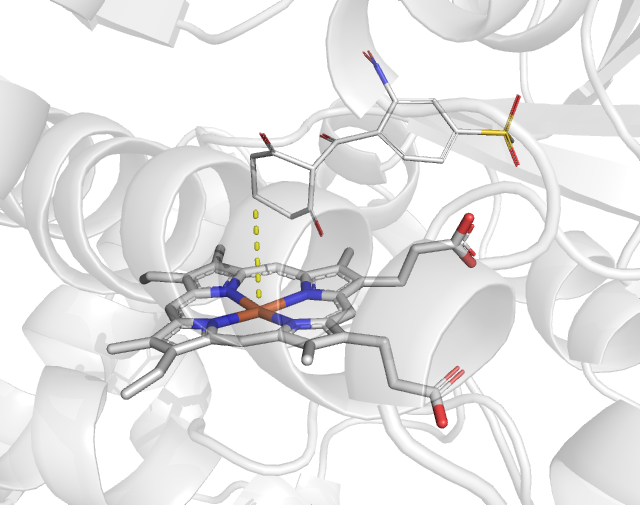
\includegraphics[width=\textwidth]{img/score.png}
	\caption{\label{score} - Distance $d$  between carbon $C_5$ of mesotrione and the heme iron of BM3, used in the fitness score (\AA) marked by a yellow dashed line.}
\end{figure}
%% to do - score functions a and b

\subsection{Genetic Algorithm \label{ga}}

A simple genetic algorithm \textit{(GA)} was used for sequence optimization during \textit{VDE}.
The \textit{GA} was implemented in pure \texttt{python} and its built-in modules.

In this case, the \textit{GA} repeated the following steps in each iteration:
\begin{enumerate}
	\item \textbf{Initialize mutant population:} From the template sequence, generate $p$ mutants each with one random point mutation.
	\item \textbf{For $n$ Iterations:}
		\begin{enumerate}
	\item \textbf{Evaluate \textit{fitness} of each mutant:\label{gaeval}} Using multiprocessing, evaluate the score for each mutant in parallel, returning a mapping of sequences to respective scores.
	\item \textbf{Select for best $\frac{1}{m}$ mutants:} where $\frac{1}{m}$ is the survival rate in each iteration.
	\item \textbf{Repopulate gene pool by crossover and point mutation of selected mutants:} where two random members of the surviving mutants $a$ and $b$ are crossed by recombining sequences at a random cut point and introducing additional random point mutation.
		Repeat $p$ times.
		\end{enumerate}
\end{enumerate}

\alglanguage{pseudocode}
\begin{algorithm}
	\caption{\label{pseudocode}: A genetic algorithm}
	\
	\begin{algorithmic}
		\Procedure{GA}{$sequence, n_{mutants}, n_{iter},n_{survivors}$} 
		\For{$i:=1; i < n_{mutants} ; i_{++}$} \Comment{Initialize a population of size $n_{mutants}$}
			\State $genePool_i := mutate(sequence)$  \Comment{Random substitution at random position}
		\EndFor
		\For{$i:=1 ; i < n_{iter} ; $} \Comment{For each generation}
			\ForAll{$mutant_j \in genePool$} \Comment{Map fitness function to each mutant}
				\State $fitness_j := fn(mutant_j)$  \Comment{where $fitness$ is mappable}
			\EndFor
			\State $genePool := nlargest(fitness,  n_{survivors}))$ \Comment{Select $n_{survivors}$ best sequences}
			\For{$i:=1 ; i < n_{mutants} ; i_{++}$} \Comment{Repopulate gene pool with new mutants}
				\State $newGenePool_i := mutate(crossover(genePool_{random}, genePool_{random}))$
			\EndFor
			\State $genePool := newGenePool$
		\EndFor
		\EndProcedure
	\end{algorithmic}
\end{algorithm}

Algorithm \ref{pseudocode} is implemented in \texttt{python} in the file \texttt{vde/ga.py} and makes use of multiprocessing to parallelise evaluations of a function.

\subsection{Main Function \label{main}}
The program in \texttt{vde/main.py} executes the main functionality of \textit{VDE}.
It executes iterations of the genetic algorithm \ref{ga} where the evaluation function for a $sequence $ is:

\begin{algorithm}
	\caption{\label{fitness}: One fitness evaluation}
	\begin{algorithmic}
		\Procedure{Evaluate Mutant}{$sequence$}
		\State structure = map\_refold(sequence, pdb=\texttt{4KEY.pdb}) \Comment{Predict mutant structure \cite{dunbrack1993backbone} \cite{chaudhury2010pyrosetta}.}
		\State docking poses = dock(structure, mesotrione) \Comment{\cite{trott2010autodock}}
		\State fitness = score(docking poses) \Comment{Using score \ref{scorefn}}
		\State \textbf{Return} fitness
		\EndProcedure
	\end{algorithmic}
\end{algorithm}

Two instances of the \textit{VDE} program were run, each with a different score function and labeled $A$ and $B$.
The score function for $A$ was as in equation \ref{scorea}:

\begin{equation}\label{scorea}
	fn_A(a, d, h) = d - \log{|a|} - h
\end{equation}

Where variables as in section \ref{scorefn}.
The score function for $B$ is described in equation \ref{scoreb}:

\begin{equation}\label{scoreb}
	fn_B(a, d, h) = (\frac{1}{n} \sum_{n}^{i} softmax(\log{|a|}_i)\times d_i) -  h
\end{equation}

Asides from the differing score functions, the two experiments were set up to be run with the configuration in table \ref{config}:

\begin{table}
        \begin{center}
		\caption{\label{config} The parameters used in experiments $A$ and $B$.}
                \begin{tabular}{l|p{3cm}}
		\textbf{Parameter} & \textbf{Value} \\
                \hline
			Template Structure & \textit{4KEY} \cite{butler2013key}\\
		Mutation Sites & 47, 49, 51, 75, 78, 88, 94, 138, 142, 175, 178, 184, 188, 205, 226, 252, 255, 260, 263, 290, 295, 328, 330, 350, 353 \\
		Population Size & 128 \\
		Survival Rate & $\frac{1}{4}$ \\
		Docking Exhaustiveness & 16 \\
		Number of Generations & 32 \\
		Number of Repeats & 8 \\
        \end{tabular}
        \end{center}
\end{table}

\begin{itemize}
	\item The \textit{Mutation Sites} were chosen manually from the crystal structure of P450 BM3 A82F/F87V mutant \texttt{4KEY} \cite{butler2013key}, the template structure for these experiments.
	\item \textit{Docking Exhaustiveness} is 16: the maximum value allowed by \textit{VINA}, which is computationally intensive but yields results with lower variability.
	\item \textit{Population Size} is 128, this was chosen because monitoring CPU usage was observed to be low in instances run with large \textit{Population Sizes} in a single process, so to maximize CPU usage, eight replicates were executed in separate parallel processes instead.

	\item \textit{Survival Rate} is $\frac{1}{4}$, where the top scoring fraction survive to repopulate the gene pool.
\end{itemize}

Experiment $A$ was run using code in the \texttt{git} branch \texttt{x2} on commit \texttt{????}, and experiment $B$ was run on branch \texttt{x3} and commit \texttt{e7af345fba8b8be36bea25982af0b978df8267e8}.

Each was run in eight parallel instances using the script \texttt{vde/vde.sh}, which launched \texttt{vde/main.py} with the command \texttt{python main.py -fn b -p 128 -e 16 -n 32 -s 0.25 \&}, which invokes the parameters in table \ref{config}.

% ---------------- cloud ----------------
\subsection{Cloud Deployment \label{cloud}}
Each \texttt{g6-dedicated-50} was provisioned with \texttt{evo/cloud/build-linode.sh} and the configuration scripts in \texttt{evo/scripts/config}.
The \textit{Linode} instance had the virtual hardware specifications showing in table \ref{linode}.

\begin{table}
        \begin{center}
		\caption{\label{linode} Virtual hardware specifications of the \texttt{g6-dedicated-50} server hired for experiments $A$ and $B$.}
                \begin{tabular}{l|p{3cm}}
		\textbf{Item} & \textbf{Specifications} \\
                \hline
			CPU cores & 50 \\
			RAM & 128 GB \\
			Disk & 250 GB \\
			Cost per hour & \$1.44 \\
        \end{tabular}
        \end{center}
\end{table}

Each experiment lasted about 3 days and cost \$103 at a rate of \$1.44 per hour. 
Data generated was structures, docking poses and scores for each mutant - it was compressed into a \texttt{.tar.gz} archive and uploaded to a \textit{Linode} bucket and the machines were terminated.

The eight replicates were run in parallel, generating 32,000 mutants for each experiment.

Data was pulled down from the bucket storage onto a separate server for analysis with specifications listed in table \ref{analysis}.
\begin{table}
        \begin{center}
		\caption{\label{analysis} Virtual hardware specifications of the \texttt{g6-dedicated-8} server hired for analysis of experiments $A$ and $B$.}
                \begin{tabular}{l|p{3cm}}
		\textbf{Item} & \textbf{Specifications} \\
                \hline
			CPU cores & 8 \\
			RAM & 16 GB \\
			Disk & 325 GB \\
			Cost per hour & \$0.18 \\
        \end{tabular}
        \end{center}
\end{table}

% ----------------
\section{Results}


\subsection{Exploratory Analysis for Experiments $A$ and $B$}
Each experiment $A$ and $B$ yielded near to 32,000 unique mutants.
The overall distributions for metrics, amino acids at each site and a set of dimensionality reduction techniques for data generated in experiments $A$ and $B$ are shown here.
These metric distributions are compared in figure \ref{abdistr}, where the recorded metrics were:
\begin{itemize}
	\item $\Delta G$: The mean binding energy for docked mesotrione poses as calculated by \textit{VINA} and given in kcal/mol.
	\item $H$: The Hamming Distance, or number of mutations relative to the wild type.
	\item $d$: The distance between mesotrione carbon $C_5$ and the heme iron, given in \AA.
	\item $score_{\in {a, b}}$: The score function $a$ or $b$ for experiments $A$ and $B$ respectively. Score $a$ is described in \ref{scorefn} and $b$ in \ref{scorefn}.
\end{itemize}

The progression of these metrics with generation for each experiment are shown in \ref{violin}.
\textbf{note:} columns mislabelled in $B$, need suptitle.
Viewing the progression of the objective score shows that for $A$ and $B$ the score distributions changed by very little, suggesting that the sequence optimization algorithm used here is a poor choice for this type of problem.
On the other hand, $\Delta G$ did increase in both, which could mean that both score functions tended to sacrifice $\Delta G$ for $H$ or $d$, or more worryingly that $\Delta G$ is prioritized and that the optimizer was unintentionally reversed.
Despite this, the algorithm did produce a large volume of data which can still be dissected to identify active mutants and gain insight. 

\begin{figure}
	\caption{\label{violin}}
\begin{subfigure}{\textwidth}
	\caption{\label{violina} Progression of $\Delta G$, $d$ and $score_a$ with generation for experiment $A$.}
	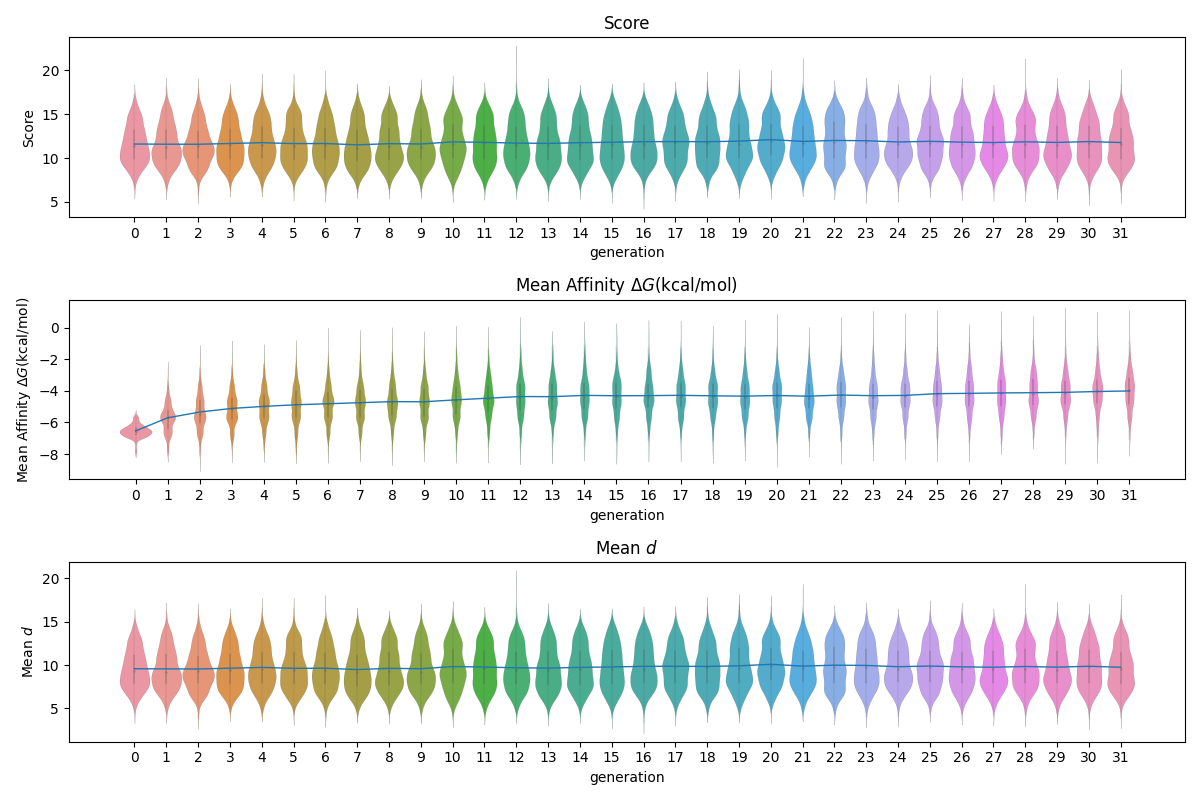
\includegraphics[width=\textwidth]{img/generation-global-dist_mean-a.png}
\end{subfigure}
\begin{subfigure}{\textwidth}
	\caption{\label{violinb} $\Delta G$, $d$ and $score_b$ with generation for experiment $B$.}
	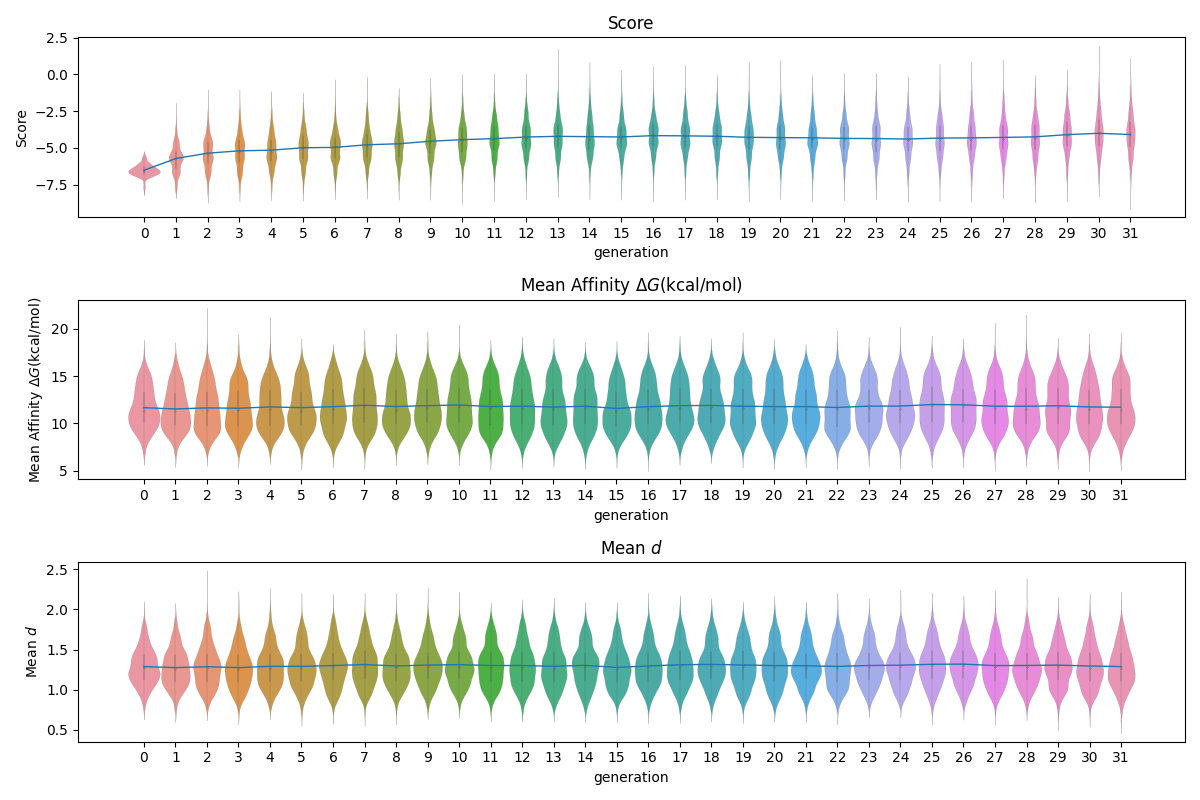
\includegraphics[width=\textwidth]{img/generation-global-dist_mean-b.png}
\end{subfigure}
\end{figure}

The histograms in figure \ref{abdistr} shows that for both $A$ and $B$, there are many mutants for whom $d < 8$ which may be suitable for the project aim.
Between the two experiments, the distance $d$ between carbon $C_5$ and the heme iron is largely similar, so too are the calculated affinities ($\Delta G$) and Hamming distance to the wild type, $h$.
Hamming distance $h$ rarely exceeded 8, likely due to the constraint on $h$ incorporated into both score functions.
Docking binding energy estimates $\Delta G$ cluster at a set of values for both experiments which may indicate the same number of pose clusters with similar energies. 
For both, distance $d$ was a skewed distribution that leans towards lower values, each with a small shoulder at around 15 \AA, which may reflect either a cluster of binding poses or a cluster of mutants for which binding of mesotrione to the active site is blocked.

\begin{figure}
	\begin{center}
		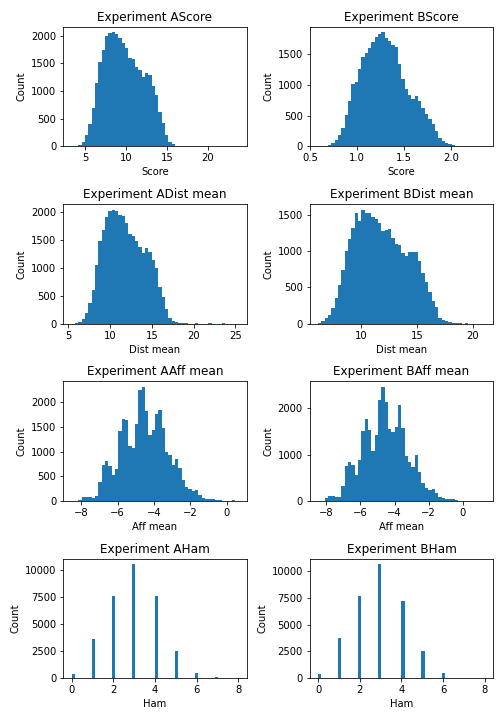
\includegraphics[width=0.7\textwidth]{img/exp-a-b-compr-dists.png}
		\caption{\label{abdistr} Histograms showing the distributions of each recorded metric across the entire experiment for both experiments $A$ and $B$.}
	\end{center}
\end{figure}

Figure \ref{logot} is a sequence logo which shows the amino acids at each mutation site for the template sequence BM3 A82F/F87V, whilst \ref{logoa} and \ref{logob} represent the overall frequencies of different amino acids across experiments $A$ and $B$ respectively.
They show that the repeats of each experiment tended towards the template amino acid at each position, likely because of the constraint on $h$ in both score functions, resulting in few mutants that are more than six mutations from the template.
Ignoring the template amino acids yields the sequences logos \ref{logonotpa} and \ref{logonotpb}, neither of which show a clear preference at any particular site.


\begin{figure}
	\caption{\label{logos} Sequence logos.}
\begin{subfigure}{\textwidth}
	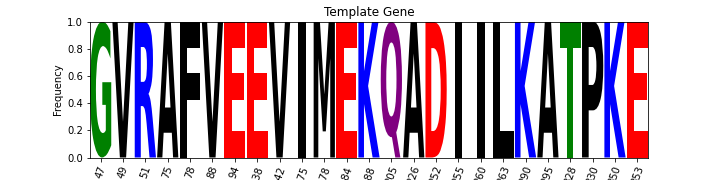
\includegraphics[width=\textwidth]{img/template-logo.png}
	\caption{\label{logot} Sequence logo showing the original amino acids at mutation positions in experiments $A$ and $B$.}
\end{subfigure}
\begin{subfigure}{\textwidth}
	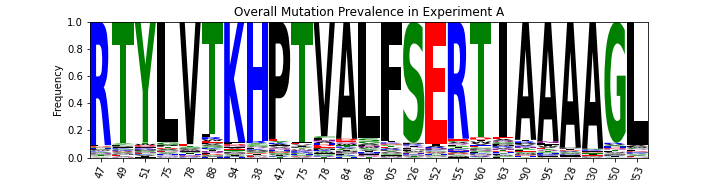
\includegraphics[width=\textwidth]{img/exp-a-logo.png}
	\caption{\label{logoa} Sequence logo showing the overall amino acid frequencies in mutants in $A$.}
\end{subfigure}
\begin{subfigure}{\textwidth}
	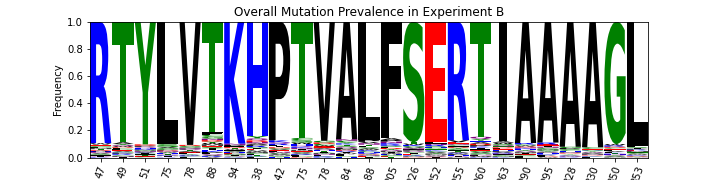
\includegraphics[width=\textwidth]{img/exp-b-logo.png}
	\caption{\label{logob} Sequence logo showing the overall amino acid frequencies in mutants in $B$.}
\end{subfigure}
\begin{subfigure}{\textwidth}
	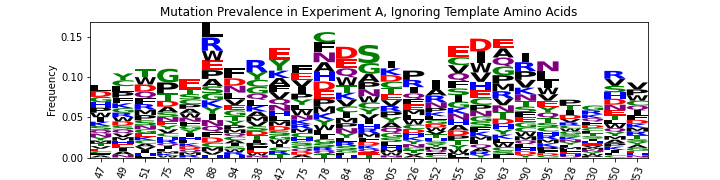
\includegraphics[width=\textwidth]{img/expa-logo-notemplate.png}
	\caption{\label{logonotpa} Sequence logo showing the bulk average mutation preference in experiment $A$, ignoring the template amino acids (\ref{logot}).}
\end{subfigure}
\begin{subfigure}{\textwidth}
	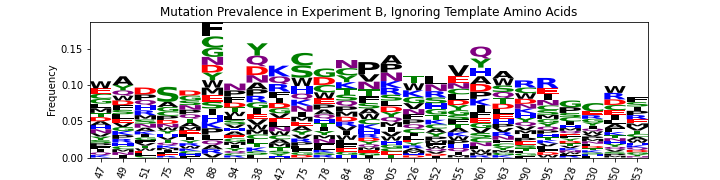
\includegraphics[width=\textwidth]{img/expb-logo-notemplate.png}
	\caption{\label{logonotpb} Sequence logo showing the bulk average mutation preference in experiment $B$, ignoring the template amino acids (\ref{logot}).}
\end{subfigure}
\end{figure}

From this we can see that the sequence optimizer has not worked, but has generated mutants predicted to have desirable mesotrione binding properties given the project aim.
Unanswered questions that remain are:
\begin{itemize}
	\item Are there clusters of sequences or regions of sequence space where desirable properties are prevalent? 
		And is there a pattern in mutation preference for these clusters?
	\item How noisy is the evaluation function?
\end{itemize}

\subsection{Clustering}

Although there was no global consensus on a set of mutations that improve binding, clusters of sequences showed improved binding properties.
Clusters of mutants were identified using dimensionality reduction and clustering algorithms.
Mutant sequences were reduced in dimensionality using both the \textit{t-SNE} \cite{van2008visualizing} and \textit{UMAP} \cite{mcinnes2018umap} algorithms to decompose an input of the binary encoded  amino acids at each mutation position.
The reduced sequence information is mapped to scores in figure \ref{dimredplt}.
% plot with metrics, hamming
%At the center of each dimensionality reduction map are the sequences that were repeatedly converged upon, visible by an area of low score (desirable).
%When colored by point density the same low scoring centers of the mapping are also densely populated.
%In order to confirm that the solutions in the centre were converged upon a generation number color map would be necessary, though was not possible since generation numbers were not recorded.

\begin{figure}
	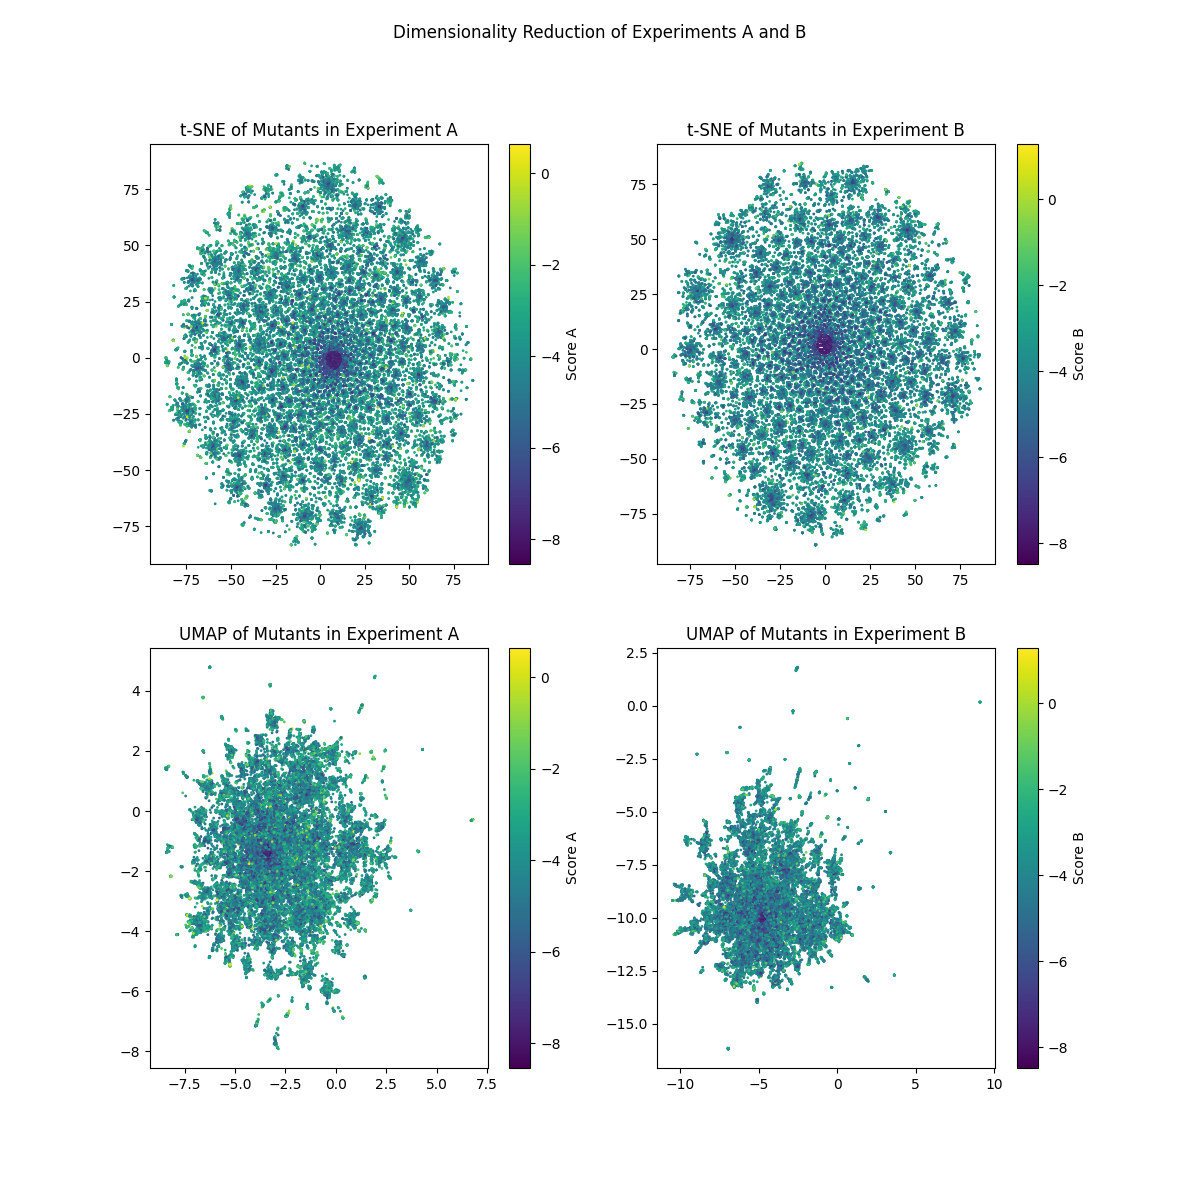
\includegraphics[width=\textwidth]{img/dimred-plt.png}
	\caption{\label{dimredplt} Two different dimensionality reduction techniques were applied to the integer encoded sequences data from $A$ and $B$.
	The coordinates are mapped to their respective scores. \textbf{note: viridis -> inferno}}
\end{figure}

\begin{center}
\begin{figure}
	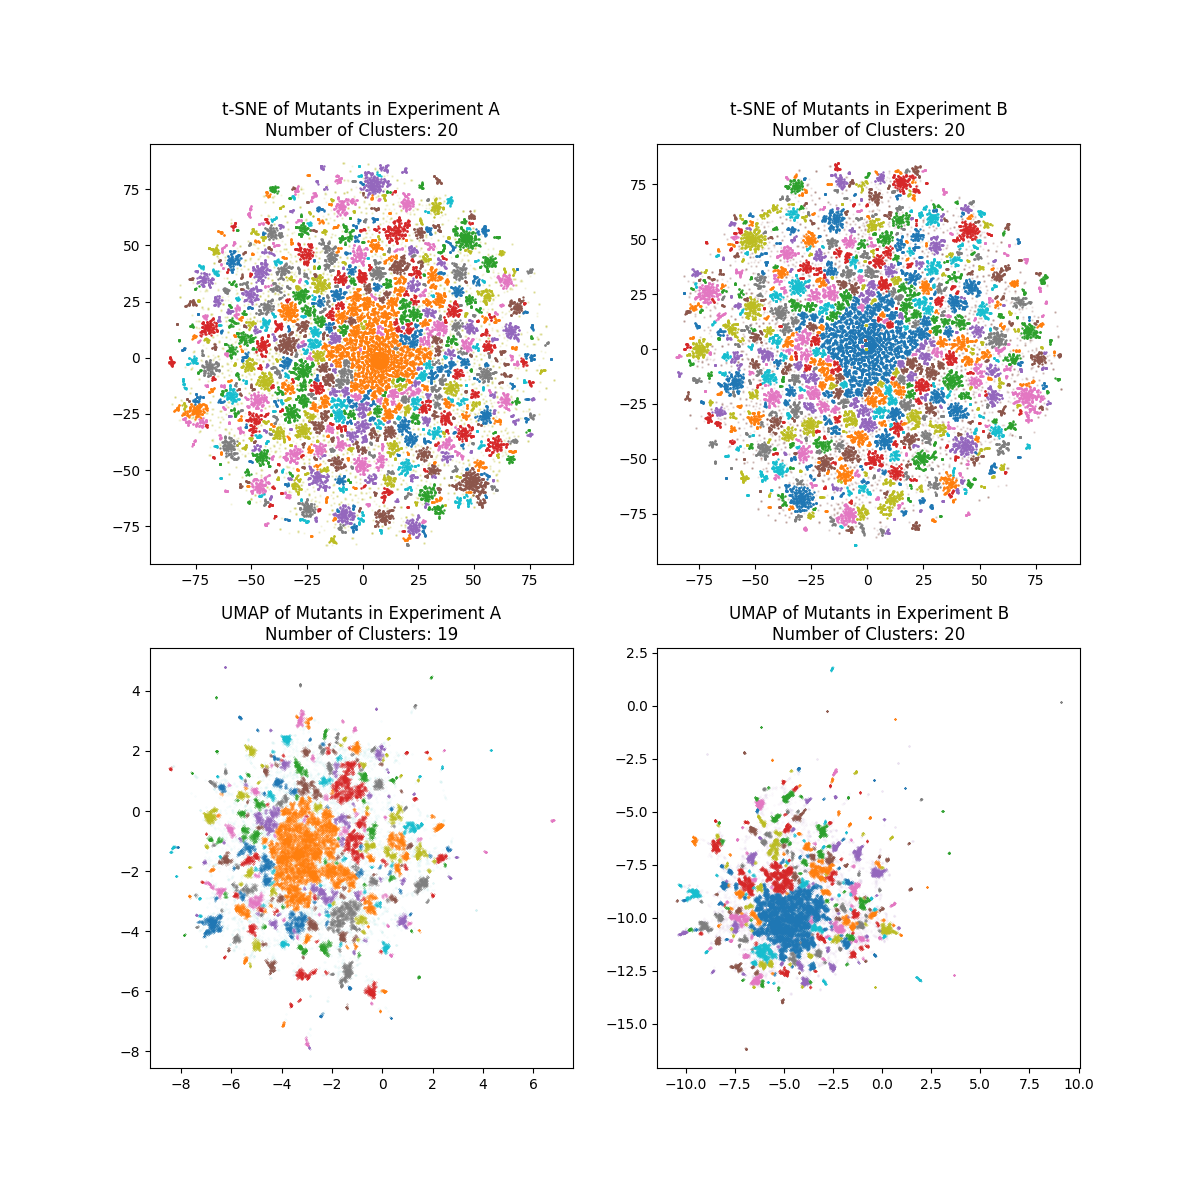
\includegraphics[width=\textwidth]{img/dimred-plt-clusters.png}
	\caption{\label{dimredclusters} The same dimensionality-reduction coordinates as in figure \ref{dimredplt} colored by cluster mapping generated by the \textit{DBSCAN} algorithm acting directly on the reduced coordinates. Color codes to clusters are not shown for the sake of space.}
\end{figure}

\begin{figure}
	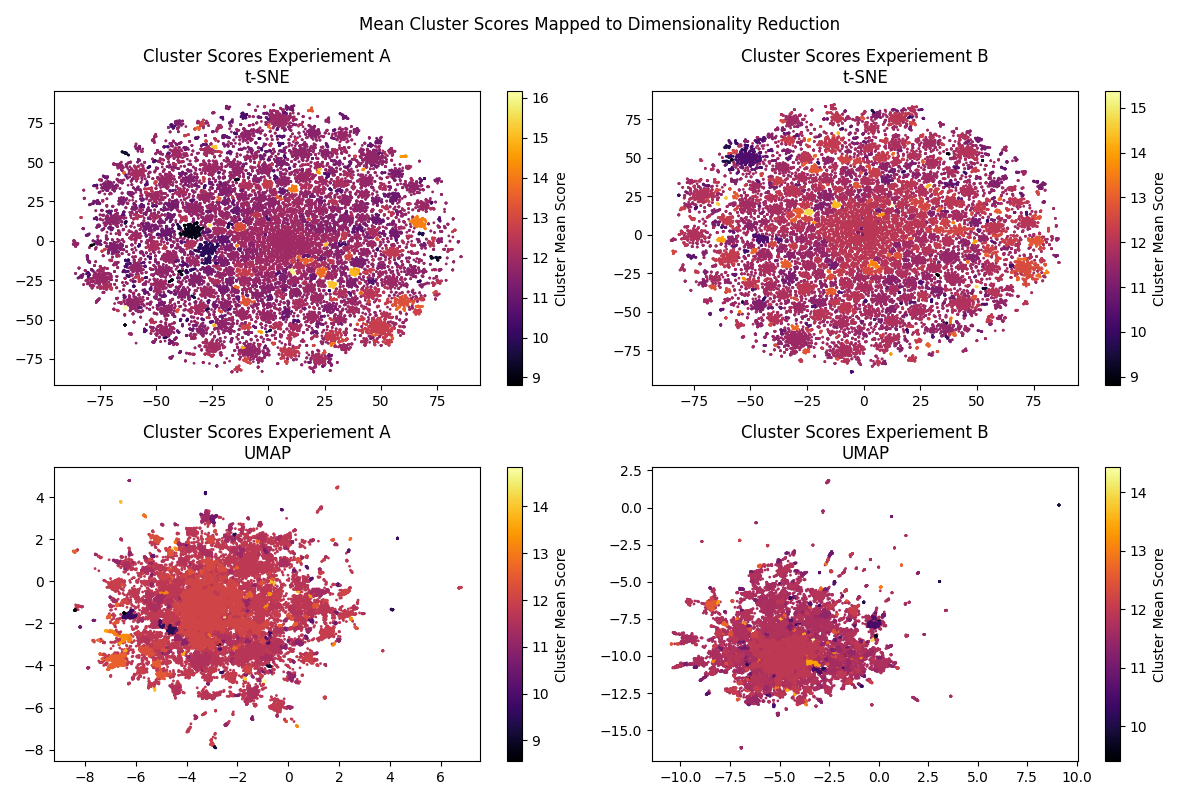
\includegraphics[width=1.1\textwidth]{img/dimred-clust-meanscores.png}
	\caption{\label{dimredclustersscores} Clusters of dimensionality-reduced mutants as in figure \ref{dimredclusters} mapped to the mean score of that cluster.
	In the t-SNE plots, clusters with high and low scores are visible in both $A$ and $B$.}
\end{figure}
\end{center}
%Whilst it is possible that the converged mutations are sufficient for creating a BM3 mutant with target activity, it is also possible that optimizing sequences for these scores exploited an inaccuracy in the model which would result in unintended consequences, such as large structural changes that can not be predicted by the model.
%To mitigate the risk of a failed round of lab screening, it is prudent to identify other clusters with activity in order to introduce diversity into the screening set.
Despite no global consensus, clusters of mutants were identified with the aim of identifying regions of sequence space with their overall favourable properties.
The hypothesis here was that some regions of sequence space would largely have similar characteristics save for extreme loss of function mutants.
Activity distributions within clusters would be different from the global distribution in this case which can be quantified using Kubrik-Leibler divergence \cite{kldiver} $D_{KL}$ in equation \ref{kldiv}.

\begin{equation}\label{kldiv}
	D_{KL}(p||q) = \sum{x \in X} p(x) \log{\frac{p(x)}{q(x)}}
\end{equation}
$KL$ divergence between two distributions $q$ and $p$ which are appropriated with the function $q(x)$ and $p(x)$ where $x$ an element of the set real numbers $X \in \mathbb{R}$.

Rather than clustering directly from the sequences, clusters were made directly from the reduced dimensions using the \textit{DBSCAN} algorithm, exemplified in figure \ref{dimredclusters}.
This was because the dimensionality reduction methods used here group spatially with similarity, so clustering spatially clusters sequences with some similar properties.
The benefits of this order of operations include performance improvements for the clustering algorithm given the lower dimensionality of the data and coherence with the sequence dimensionality reduction which makes it useful as a \textit{fitness map}.

For each dimensionality reduction technique, \textit{DBSCAN} was used to identify clusters from the coordinates, shown in figure \ref{dimredclusters}.


\subsection{Codon Design}
From these clusters, the best scoring eight were selected, their amino acid frequencies calculated and degenerate codons designed to reflect that frequency using the \textit{Codon Genie API}.
Reports for each were generated and an example is shown in figure \ref{cdxreport} and the codons designed for exemplary cluster 314 are in table \ref{cdx314}.

\begin{table}
\caption{\label{cdx314} An example of the codons auto-generated for mutant cluster 314, which encodes few variants. 
	A total of 1024 variants are encoded by this set of codons. }
\begin{tabular}{lllcl} 
	\textbf{Position} & \textbf{Codon} & \textbf{Expansion} & \textbf{Number of Encoded Variants} & \textbf{Amino Acids} \\
	\hline
	47  &   CGT &  CGT &       1 &  R \\
	49  &   ACC &  ACC &       1 &  T \\
	51  &   TAT &  TAT &       1 &  Y \\
	75  &   CTG &  CTG &       1 &  L \\
	78  &   GTT &  GTT &       1 &  V \\
	88  &   WSG &  ACG, AGG, TCG, TGG &             4 &  T, W, R, S \\
	94  &   AAA &  AAA &       1 &  K \\
	138 &   CAT &  CAT &       1 &  H \\
	142 &   GGT &  GGT &       1 &  G \\
	175 &   ACC &  ACC &       1 &  T \\
	178 &   GTT &  GTT &       1 &  V \\
	184 &   KMT &  GAT, GCT, TAT, TCT &             4 &  A, Y, D, S \\
	188 &   CTG &  CTG &       1 &  L \\
	205 &   TTT &  TTT &       1 &  F \\
	226 &   AGC &  AGC &       1 &  S \\
	252 &   GAA &  GAA &       1 &  E \\
	255 &   CAG &  CAG &       1 &  Q \\
	260 &   ACC &  ACC &       1 &  T \\
	263 &   MRT &  AAT, AGT, CAT, CGT &             4 &  N, R, H, S \\
	290 &   RMT &  AAT, ACT, GAT, GCT &             4 &  A, N, D, T \\
	295 &   GCA &  GCA &       1 &  A \\
	328 &   GCA &  GCA &       1 &  A \\
	330 &   RMA &  AAA, ACA, GAA, GCA &             4 &  A, K, E, T \\
	350 &   GGT &  GGT &       1 &  G \\
	353 &   CTG &  CTG &       1 &  L \\
\end{tabular}
\end{table}

This way, codons were designed for clusters in experiments $A$ and $B$, the data and reports for which are stored in \texttt{nb/codons/} of the project \texttt{git}  repository.
The total size of each library yielded by the codon design varies from four to several thousand, the latter of which are not suitable for use owing to the extreme numbers of potential variants.
Some libraries also inadvertently encode a \textit{Stop} codon, which should also be avoided.


\begin{figure}
\begin{subfigure}{\textwidth}
	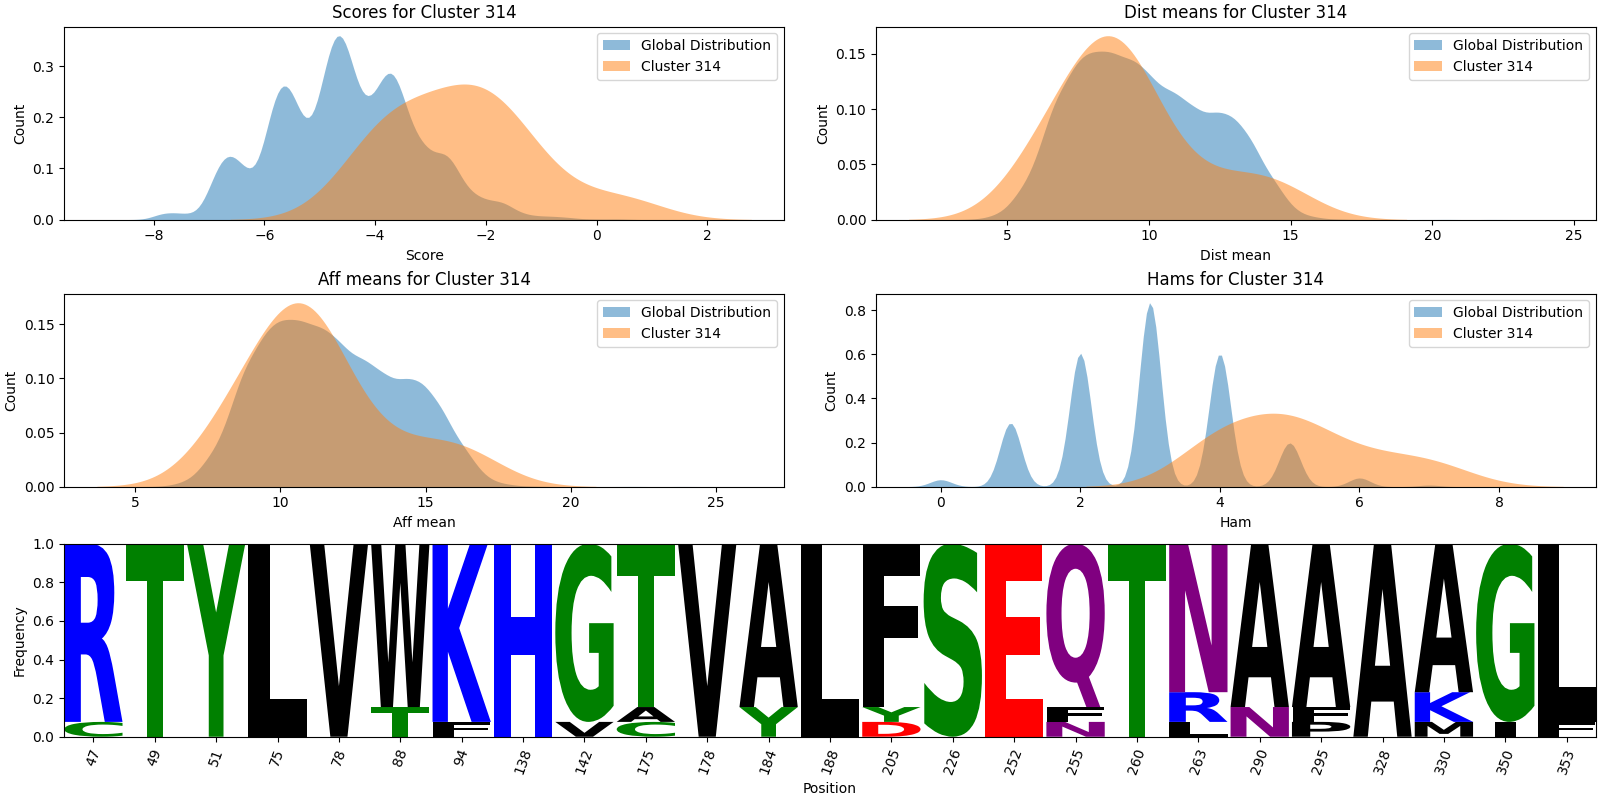
\includegraphics[width=\textwidth]{img/clus_314.png}
	\caption{\label{cdxreport} A codon report for cluster 314 derived from a \textit{UMAP} of the sequences in experiment $A$.
		 Shown are the cluster distributions of each recorded metric relative to the global distribution.
		 The sequence logo represents the mutation frequency at each position. \textbf{note: map back to umap}}
\end{subfigure}
\begin{subfigure}{\textwidth}
	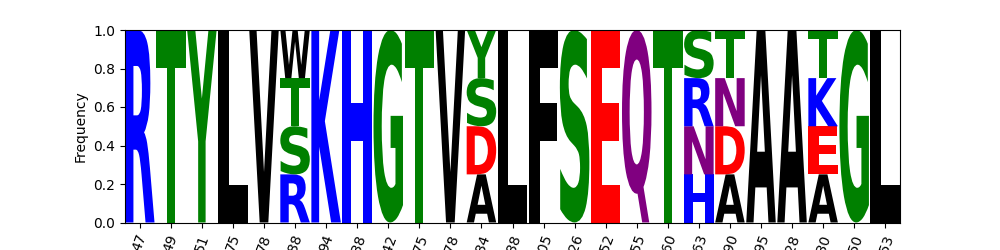
\includegraphics[width=\textwidth]{img/clus_314-codon-coverage.png}
	\caption{\label{cdxreportcoverage} The amino acid coverage of the degenerate codons designed for cluster 314, which include off-target amino acids at several sites.}
\end{subfigure}
\end{figure}

% ----------------
\section{Discussion and Future Work}

Here, a working \textit{Virtual Directed Evolution} system was developed, including the simulation back end \texttt{enz}.
The system used a genetic algorithm to optimize a set of mutation points in the Cytochrome P450 BM3 for a mesotrione binding metric that aimed to select for mutants that dock mesotrione with the $C_5$ carbon of mesotrione held stably near the BM3 heme iron.
It was run on cloud infrastructure at a scale of 64,000 mutants over a three day period.
From the output of the algorithm a set of mutations with potentially desirable effects were identified, given the aim of engineering a BM3 mutant capable of mesotrione 5-hydroxylation.
Additionally, mutant clusters were found amongst the results of the algorithm, for the most active of which sets of degenerate codons were designed.

The system was designed to be modular enough so that components can be modified independently of one another.
As such it is important to review these components with a view to fixing and upgrading them.

The most critical uncertainty and potential shortcoming of this implementation of \textit{Virtual Directed Evolution} is whether the simulation evaluation used is a meaningful metric to optimize for.
The accuracy of the simulation in portraying relevant aspects of the enzyme-ligand interaction is critical to be applicable to the world outside the simulation.
So too is the meaningfulness of the score function which is to be optimized for, which in this case is only designed as a proxy to desired chemical activity.

Less critical, though with operational significance is the efficacy and efficiency of the sequence optimization algorithm used.
Large gene pools improve the performance of genetic algorithms, so scale is important.
Slightly out of scope of \textit{Virtual Directed Evolution} is codon design, which must yield libraries that are small enough to screening and rich enough in activity to offset the high cost of making and testing the mutants.

These key parts of the project are dissected further for potential improvements:

\subsubsection{Simulation Accuracy}
In as far as a simulation is a time series approximation of a real world situation, the simulation here is a misnomer for referring to prediction of mutant structures and likely binding poses between them and mesotrione before being subject to some score function.
That said, the simulation used in this work is crude owing to its lack of protein backbone movement during structure prediction and lack of interaction dynamics between protein and ligand.
These two functions, protein structure prediction and docking were contained by \texttt{enz}, which abstracts these two functions in its \textit{API} and therefore the scope of improvements to simulation accuracy are within \texttt{enz}.

There are several aspects of \texttt{enz} that can be improved over different time scales.
One short and simple improvement is unit testing of all code in the module to ensure that the code behaves as expected.
There is currently no unit testing in \texttt{enz} which limits the ability to diagnose problems with it.

Since \texttt{enz} itself is a simple wrapper around protein structure prediction and docking programs, those programs can be replaced or modified.
\textit{PyRosetta} proved problematic in deployment owing to its licensing and package size, which necessitates distribution of \textit{PyRosetta} to target machines via direct file transfer as opposed to download directly from the world wide web.
This was done here by storage of a copy in a \textit{Linode} bucket storage in Hamburg which itself required authentication with the \texttt{linode-cli} interface, a step that would require careful planning were it to be fully automated given that access tokens would be in play.

\textit{PyRosetta} contains lots of functionality, but only a single function - side chain repacking \cite{dunbrack1993backbone} is used. 
Cyclic coordinate descent as a means of predicting loop structure \cite{canutescu2003cyclic} was investigated but subsequently dropped owing to the difficulty of the software implementation, which would often result in \textit{Segmentation Faults} that crash the process by attempting to access out of bounds memory, something inherent to \textit{PyRosetta} itself.
\textit{Segmentation Faults} were commonplace in investigating other folding methods, which combined with sparse documentation coverage and a license which incurs an annual cost to non-academic users raises a case for exploring other protein folding methods.

Recent advances in the use of machine learning in protein structure prediction \cite{jumper2021highly} have outperformed their non-learning counterparts.
Though the \textit{de-novo} structure prediction of \textit{Alphafold} \cite{jumper2021highly} outperforms all known structure prediction methods to date, since it is such a large model it requires GPU or TPU cores to function and may take some hours on a single prediction. 
\textit{De-novo} protein structure prediction may be unnecessary for this application, since the protein backbone chain may be similar among mutants.

Template-based protein structure prediction using machine learning methods may on the other hand be more viable, given the shorter prediction times involved.
An additional advantage of using a lightweight machine learning-based method is the prospect that inference can be accelerated significantly using a GPU or TPU.
One candidate for replacement of the \textit{PyRosetta} back end is \texttt{torchmd} \cite{doerr2021torchmd}: an open-source \textit{PyTorch}-based molecular dynamics package which would allow side chain replacement and subsequent repacking via either energy minimization using a force field such as \textit{Amber}\cite{wang2004development}.
Being based on \textit{PyTorch}, there is scope for accelerated calculations using GPUs, and it also offers compatibility with other \textit{PyTorch}-implemented protein structure machine learning methods.

Docking using \textit{VINA} is CPU-bound and the most time-consuming step of each round of the \textit{Virtual Directed Evolution}.
This can be accelerated with more CPU cores, or employment of a GPU-based docking program like \textit{Autodock GPU}\cite{santos2021accelerating}, which is free and open source.
Alternatively, emerging docking methods based on machine learning may be worth consideration given their performance \cite{doerr2021torchmd}; should these methods be implemented in \textit{PyTorch} then the entire protein structure prediction and docking pipeline could be carried out on a GPU without writing to disk or converting file formants.

The structure of the \texttt{enz} wrapper allows for drop in replacements of each component, whilst also providing a coherent data structure for user interaction and analysis which is essential for scoring.
The key priorities for improvements to \texttt{enz} are:

\begin{itemize}
	\item \textbf{Accuracy:} To assess accuracy, a task-relevant baseline needs to be established. 
		In the context of an enzyme engineering project, this could be the results of a lab screen of the mutants generated here.
		In that case, correlation between simulation predictions and lab metrics can be quantified using an appropriate metric like Pearson's correlation coefficient. 
		With a metric to optimize towards, changes can be made to the underlying simulation mechanisms of \texttt{enz}.
		An alternative, cheaper source of baseline data is the \textit{PDBBind}\cite{liu2015pdb} dataset - a collection of ligand bound protein structures for which the task would be to replicate these bound configurations using docking.
		Differences between poses generated by docking and those in the \textit{PDBBind} dataset can be quantified using a metric like root mean squared difference (RMSD) between each atom.
		
	\item \textbf{Performance:} Both \textit{PyRosetta} and \textit{VINA} are CPU-bound, which limits the speed at which mutants can be evaluated because of the inherently linear nature of CPU processing. 
		Should alternatives for both be found they would ideally run with GPU acceleration, which is inherently parallel.
		\textit{Autodock GPU}\cite{santos2021accelerating} is an attractive short-term replacement for \textit{VINA} given its performance. 
		Beyond short term changes, structure prediction and docking algorithms implemented in \textit{PyTorch} are attractive because of the prospective GPU acceleration and compatibility with machine learning algorithms.
	\item \textbf{Portability:} Installing the required environment on the target machine with minimal intervention is important for scaling to multiple machines.
		Therefore, the \textit{portability} of the requirements - in terms of ease of data automated data transfer and setup is important.
		\textit{PyRosetta} is not free for non-academic users, which makes it more difficult to find on the clear web and is a reason to not use it in a commercial setting.
		It also relies on distribution of compiled binaries that may not be suitable for a particular CPU architecture or operating system.
		It is also large - with the compressed release reaching 1.3 GB, which is uncomfortably large given that only a small subset of its functionality are employed.
\end{itemize}

\subsubsection{Score Relevance}
 The score function optimized towards during runtime is critical for output of mutants with the desired activity in the real world.
 It uses a set of assumptions as a proxy metric for likelihood of $C_5$ mesotrione hydroxylation:
 \begin{enumerate}
	\item That the $C_5$-heme iron distance $d$ must be minimized in order to maximize the likelihood of the desired reaction.
	      This is based on the assumption that $C_5$-heme iron proximity will drive the target reaction.
	      It also assumes that the chemical potential between the two atoms is sufficient to drive electron transfer from the BM3 reductase domain to $C_5$.
	\item That the estimated binding $\Delta G$ energy of a pose to BM3 relates to the likelihood of that pose occurring. 
	\item That a low Hamming distance $h$ between a mutant sequence and the template indicates that the mutant structure would not be so different from the template that the protein structure prediction methods used are sufficiently accurate.
 \end{enumerate}

If these assumptions hold, then the score function may be sufficient as is in experiments $A$ and $B$.
The ideal scenario for evaluating the efficacy of the score function is to compare it to lab data containing BM3 mutants and data on the products formed on reaction with mesotrione, if any and the rate at which they are formed.

Since the score is only a simple proxy in its current states, in future design iterations in conjunction with lab data to mimic it will likely grow in complexity.

\subsubsection{Sequence Optimization}

Though a genetic algorithm was used as a sequence optimizer in this work, others can be used and the genetic algorithm itself stands to be modified to improve efficiency.
A genetic algorithm was implemented because they are simple and inherently parallelisable, which suits horizontal scaling of processes.
Many evolutionary algorithms have been studied in other work, which represents a rich field from which to harvest upgrades.

Some changes that can be made include:
\begin{itemize}
	\item \textbf{Tournament Selection:} Rather than selection of the $n$ best performing mutants, random pairs are compared for score and the best performing survives.
		This introduces an element of randomness which can enhance diversity and avoid \textit{local minima trapping}, where a good solution is found in a small subset of sequence space but is far from the global optimum for the given constraints.
	\item \textbf{Randomness:} As with tournament selection, an element of randomness in the selection step can help avoid \textit{local minima trapping} in a similar manner to tournament selection.
	\item \textbf{Generation Persistence:} The implementation used here only carries the current generation in memory, so if a cluster of good mutants are found in an earlier round there is a risk of \textit{forgetting} by evolutionary divergence from those sequences. 
		A solution to this could be that the best performing mutants within and between experiments are cached and repopulation stems from this pool.
\end{itemize}

Again, a benchmark for performance of these algorithms must be established to update and improve it.
The benchmark must be task relevant in that it approximates the type of fitness landscape expected for protein sequence optimization, so it may be best done with the current simulation method.
In this case, the metric for improvement can be some formulation of:

\begin{itemize}
	\item Rate of fitness improvement $\frac{\delta f}{\delta t}$, where the area under an curve interpolated through points of generation numbers against fitness scores can represent this rate.
		Alternatively, the initial gradient of the interpolated curve may also be a suitable metric for rate of fitness improvement.
	\item Maximum fitness attained by the algorithm may be a good indicator of whether the algorithm is subject to \textit{local minima trapping}, which itself may be a good proxy metric for sequence exploration.
	\item Exploration of new sequences is important to avoid \textit{local minima trapping} and to avoid re-visiting sequences.
		This can be quantified using a sequence diversity metric of all mutants tested over the course of an experiment, such as the sum of pairwise $h$ between all sequences.
\end{itemize}

Many improvements within the scope of the implemented genetic algorithm stand to be investigated, other sequence optimization algorithms are worth investigation.
Namely, \textit{Bayesian Optimization} is an attractive candidate for this given its efficiency and applicability to sequence optimization.
\textit{Bayesian Optimization} uses an internal \textit{Bayesian} model of response to action space input in order to generate new inputs based on their expected fitness  $\mathbb{E} f$ and expected information gain $\mathbb{E}IG$.

\subsubsection{Scale}

Scale is important to evolutionary algorithms, where a large gene pool in each generation leads to more diversity explored.
Even using \textit{Bayesian Optimization}, a large batch of candidates evaluated in parallel will likely yield a solution faster than sequential evaluations.
Therefore, scaling to a large number of parallel evaluations is important.
Using cloud resources is ideal for rapid and elastic scaling, where instances are provisioned for the duration of the experiment and then terminated, reducing costs massively compared to the overhead cost of purchasing and maintaining the equivalent computing hardware.
It also allows immediate scale to $n$ machines with $m$ computing cores.

That said, in this work the algorithm was run on a single, large machine which tool some semi manual setup using a set of scripts included in this repository.
Scripts were required because inclusion of \textit{PyRosetta} in the project would push the size of a disk image of the machine above the upper limit of that allowed to be saved, stored and distributed using \textit{Linode}.
Were this process able to boot directly from a disk image, setup could be fast and automated.

To increase scale beyond that used in this project, each round of evaluations may have to be distributed among multiple machines.
This can be done using a hub and spokes model where the sequence optimization algorithm resides in the hub node and the more expensive evaluations are sent to the spoke nodes.
This can be coordinated using the \textit{Kubernetes} engine, which is designed to orchestrate and distribute jobs amongst an array of virtual machines.
\textit{Kubernetes} can then be used for arbitrary horizontal scaling and coordination of clusters of machines.

\subsubsection{Codon Design}

Though slightly out of scope of \textit{Virtual Directed Evolution} itself, efficient codon design is essential for downstream applications.
Here several sets of codons were designed for downstream experiments in the lab, the results of which can be used to improve the algorithm.
Codons were designed as degenerates, each potentially encoding a selection of amino acids.

An important consideration in codon design are the library size, which can be calculated by taking the product of the number of amino acids that each degenerate codon  encodes.
Library size constraints are determined by the capacity of downstream screening or selection processes.
If screening based on colonies picked from the transformed libraries is used then the cost of the screen scales with the number of mutants, in which case a library size on the order of hundreds may be advisable.
On the other hand if the downstream process is a selection screen, then constraint on library size may be imposed by the transformation efficacy into the selection cells, which may be on the order of 10\textsuperscript{4}, though repeating transformations and subsequent selection steps can be cheap, so a library size on the order of 10\textsuperscript{5} may be suitable.

Although the codons themselves are designed here, no additional designs towards DNA assembly are made, for example primer design.
Should this functionality be improved, it represents project creep and will best be compartmentalized within another project.

\printbibliography
\end{document}
